\documentclass[11pt]{article}

% ---------- Packages ----------
\usepackage[margin=1in]{geometry}
\usepackage{graphicx}
\usepackage{amsmath}
\usepackage{amssymb}
\usepackage{booktabs}
\usepackage{caption}
\usepackage[colorlinks=true, linkcolor=blue, citecolor=blue, urlcolor=blue]{hyperref}
\usepackage{xcolor}
\usepackage{parskip}
\usepackage{enumitem}
\usepackage{fancyhdr}
\usepackage{titling}

% ---------- Header/footer ----------
\pagestyle{fancy}
\fancyhf{}
\fancyhead[L]{\small AvalancheBreak Project --- UC Davis Quon Lab}
\fancyhead[R]{\small\thepage}
\renewcommand{\headrulewidth}{0.4pt}

% ---------- Title ----------
\title{\textbf{Do Structural Boundary Tokens Delay the Accuracy Cliff?}\\[4pt]
\large A multi-model replication and extension, with a corrected pipeline}
\author{AvalancheBreak Project \\ UC Davis Quon Lab}
\date{}

\begin{document}

\maketitle
\thispagestyle{fancy}

\begin{abstract}
\noindent
Large language models exhibit a sharp \emph{accuracy cliff} on deterministic, multi-step tasks: performance holds up over short sequences and then collapses well before any obvious capacity limit. A recent line of work models this collapse using a Sherrington--Kirkpatrick (SK) spin-glass framework, in which an \emph{error-accumulation factor} $\alpha > 1$ produces runaway compounding of mistakes, and proposes a single-pass mitigation: inserting periodic structural boundary tokens (\texttt{|}) into the input to interrupt attention-driven error cascades. We replicate this proposal from scratch on three open-weight instruction-tuned models (Qwen2.5-7B, Qwen2.5-14B, Mistral-7B-v0.3), and extend it with a full statistical sweep, an expanded boundary-density grid, cross-model validation, and a 20-trial-averaged mechanistic analysis of attention.

We find the core claim holds, but only under a scope condition the original framing does not state: on the simplest version of the task (a 2-symbol alphabet), boundaries reduce $\alpha$ substantially and consistently in all three models --- the cleanest, most reproducible effect in this study. On harder variants (4- and 8-symbol alphabets), the effect is inconsistent across models --- present in one, reversed in another --- and should not be reported as a general property of the intervention. We confirm the proposed mechanism directly: boundary tokens act as measurable attention sinks ($R^2 \geq 0.98$ across a 20-trial sweep), attention entropy rises under boundaries in 360 of 360 sampled trials, and letter-to-letter attention measurably dips at exactly the token distances boundaries introduce. Beyond this correlational picture, a causal intervention confirms the mechanism is load-bearing, not merely associated with the benefit: zeroing attention to boundary tokens for just the 10 heads (of 784) that attend to them most erases up to 62.6\% of Cellular's accuracy benefit over Base, with the effect growing monotonically with sequence length. We also report a clean negative result: on integer addition, a task with genuine right-to-left carry dependency, boundaries make performance \emph{worse}, not better, at every tested length --- evidence that the intervention helps specifically when a task's per-position outputs are independent, and can actively hurt when they are not. Finally, we document and correct a methodological bug present throughout the original pipeline --- evaluating an instruction-tuned model without its chat template --- and show that fixing it materially changes results for at least one condition (an 8-symbol alphabet), which we flag as a general caution for future work in this area.
\end{abstract}

\section{Introduction}

Ask a language model to perform a simple, fully deterministic transformation --- shift every character forward in a fixed alphabet, keep a running sum modulo $M$, add two numbers --- and accuracy does not degrade the way one might expect. It does not fade smoothly as the input gets longer. It holds up close to ceiling, then falls off a cliff.

This is not simply the model ``running out of capacity.'' Recent work modeling this phenomenon (Hou et al., arXiv:2511.00763) casts it in the language of a Sherrington--Kirkpatrick spin-glass: the whole-sequence success rate follows

\begin{equation}
\text{SAR}(N) = \exp\left(-\beta_0 \cdot N \cdot \alpha^{N-1}\right)
\end{equation}

where $\beta_0$ is the intrinsic per-token error rate and $\alpha$ is an \textbf{error-accumulation factor}. When $\alpha = 1$, errors are independent across positions and accuracy decays as ordinary exponential decay --- a slope. When $\alpha > 1$, each error raises the probability of the next, and the result is a cliff: a sequence length $N^*$ beyond which success collapses almost completely, computable directly from $\beta_0$ and $\alpha$.

A companion proposal, \emph{``Keeping LLMs Focused: Delaying Error Avalanches via Structural Boundaries,''} argues that periodically inserting a structural marker token (e.g.\ \texttt{|}) into the input --- with instructions to copy it through unchanged --- measurably reduces $\alpha$, without requiring the multiple independent model calls that a true divide-and-conquer approach would need. The mechanism proposed: boundary tokens become \textbf{attention sinks}, absorbing attention that would otherwise flow from a token to distant, possibly-already-wrong context, thereby containing errors rather than letting them propagate.

This paper is an independent, from-scratch replication and stress-test of that proposal. We test it across three models spanning two architecture families and two parameter scales; we extend the boundary-density grid; we run every attention-mechanism claim as a genuine multi-trial statistical estimate rather than a single illustrative example; and --- critically --- we found and corrected a methodological bug in our own initial pipeline (evaluating an instruction-tuned model without its chat template) that materially changed results for at least one tested condition. We report where the effect is robust, where it is not, and where a plausible mechanistic story turned out to need a real caveat once we checked it against more than one anecdote.

\subsection{Related work}

The attention-sink mechanism this paper investigates is not a new observation in isolation --- it connects to several adjacent literatures this paper had not previously situated itself against. \textbf{Attention sinks} were first characterized as a general phenomenon by Xiao et al. (StreamingLLM, arXiv:2309.17453), who found that LLMs allocate disproportionate attention to a small number of tokens --- canonically the first few tokens of a sequence --- regardless of their semantic content, and that preserving these tokens' KV cache is sufficient to stabilize streaming generation over very long contexts. Follow-up work has shown the same phenomenon extends to \textbf{delimiter and separator tokens} specifically: SepLLM (arXiv:2412.12094) shows that ordinary segment separators accumulate outsized attention mass and can be exploited to compress a segment's information into its separator token for efficient inference, and a broader empirical survey (arXiv:2410.10781) documents when and why sink behavior emerges over training. Our Section~\ref{sec:attention-sinks} finding --- that boundary tokens inserted specifically for this purpose become measurable attention sinks, with mass that grows with density and (more slowly) with sequence length --- is best read as a targeted, causally-tested instance of this general phenomenon, applied deliberately as an error-mitigation intervention rather than observed as an efficiency side effect.

This also connects to \textbf{mechanistic interpretability of attention-head function}. Olsson et al. (arXiv:2209.11895) identify \emph{induction heads} --- head pairs that implement a ``complete the pattern [A][B]...[A]$\to$[B]'' copying operation, whose emergence coincides with a sharp jump in a model's in-context-learning ability. Our causal ablation (Section~\ref{sec:causal-ablation}) identifies a small, specific set of heads as functionally load-bearing for the boundary-token benefit; whether these heads overlap with, or are functionally related to, induction heads is a natural question this paper had not previously tested directly.

Separately, \textbf{``lost in the middle''} (Liu et al., arXiv:2307.03172) documents that LLM accuracy on long-context retrieval degrades specifically for information placed in the middle of a context, U-shaped around a strong preference for the start and end. That work and this one both concern position-dependent failure in long inputs, but via different mechanisms and mitigations: lost-in-the-middle is about \emph{where} relevant information sits in an otherwise unstructured context, while the boundary-token intervention is about \emph{periodically restructuring} the whole context regardless of where the informative content sits --- the two failure modes are plausibly complementary rather than competing explanations of long-context degradation.

Finally, this work sits alongside --- rather than in competition with --- explicit \textbf{decomposition-based prompting} strategies: least-to-most prompting (Zhou et al., arXiv:2205.10625) and program-of-thoughts (Chen et al., arXiv:2211.12588) both address error accumulation on multi-step tasks by decomposing a problem into sub-steps solved (semi-)independently, closer in spirit to this paper's own true divide-and-conquer baseline (Section~\ref{sec:divide-conquer}) than to the single-pass boundary-token intervention. Our direct empirical comparison in Section~\ref{sec:divide-conquer} --- true divide-and-conquer wins on accuracy at every tested length but costs 3--4$\times$ more compute by $N=64$ --- can be read as a quantified version of the tradeoff these decomposition strategies are implicitly making: more calls, more accuracy, at a real and growing cost that boundary tokens partially and cheaply approximate in a single pass.

\section{Methods}

\subsection{Task design}

The primary task is \textbf{cyclic character shift}: given an alphabet of size $A \in \{2, 4, 8\}$, a random string of length $N$ is sampled uniformly, and the model must replace every character with the next one in the alphabet (wrapping around). In the \textbf{Base} condition the model receives the raw string. In the \textbf{Cellular} condition, a \texttt{|} marker is inserted every $k$ characters (boundary interval $k$); the model is instructed that \texttt{|} carries no meaning and must be copied through unchanged. Boundary density is reported as $1/k$ (0 for Base).

Two secondary tasks probe whether the mechanism depends on a task's information structure: \textbf{running-sum-mod-$M$}, where each output digit genuinely depends on the cumulative sum of every prior digit (true global state), and \textbf{integer addition}, where correctness depends on carries propagating right-to-left --- the opposite direction from left-to-right generation.

Two accuracy metrics are used throughout: \textbf{TAR} (Total token Accuracy Rate, i.e.\ per-character accuracy) and \textbf{SAR} (Sequence Accuracy Rate, i.e.\ whole-sequence exact match --- an unforgiving all-or-nothing metric that collapses to floor much faster than TAR as $N$ grows).

\subsection{Models}

Three instruction-tuned models were evaluated on the full experimental battery: \textbf{Qwen2.5-7B-Instruct}, \textbf{Qwen2.5-14B-Instruct} (same family, larger scale), and \textbf{Mistral-7B-Instruct-v0.3} (different architecture family, matched parameter scale to the 7B Qwen model). This design separates ``does the effect survive scaling'' from ``does the effect survive a change of architecture.'' A fourth family, Phi-3.5-mini-instruct, was later run on the headline grid alone as an additional scope check (Section~\ref{sec:fourth-model}).

\subsection{A methodological correction: chat templates}

Every model here is instruction-tuned, and the Hugging Face / model-card documentation for each specifies a required chat template (special tokens wrapping the user turn) for correct behavior. Our initial pipeline --- and, as far as we can tell from the artifact available to us, the original draft this project replicates --- fed the model raw, unwrapped prompt text instead. This is a documented requirement, not a stylistic choice.

We reran the full grid with \texttt{tokenizer.apply\_chat\_template(..., add\_generation\_prompt=True)} applied correctly and compared. The correction closed most of the gap between our reruns and the original draft's reported numbers, and for at least one condition (8-symbol alphabet, mid-range sequence lengths) it changed results substantially: raw-text prompting produced noisy, inconsistent behavior for that alphabet specifically, which resolved into a much smoother, more interpretable trend once the model was prompted in its expected format (Figure~\ref{fig:fig8}). We flag this as a general caution: evaluating an instruction-tuned model outside its trained prompt format does not add noise uniformly across conditions --- it can distort some conditions much more than others, which is exactly the kind of confound that could be mistaken for a genuine experimental effect.

All results reported below use the corrected, chat-templated pipeline unless explicitly noted otherwise (Figure~\ref{fig:fig8} shows both, by design, to make the size of the correction visible).

\subsection{Statistical methodology}

Every accuracy condition (model $\times$ alphabet $\times$ interval $\times$ length) is run for 20 independent trials with fresh random sequences, and every reported error bar is the \textbf{standard error of the mean} (std$/\sqrt{20}$), not raw standard deviation --- we found and corrected an early version of several figures that plotted raw std, which for a near-binary metric like TAR/SAR overstates uncertainty in the plotted mean by roughly 4--5$\times$.

The SK model ($\beta_0$, $\alpha$) is fit via bounded nonlinear least squares (\texttt{scipy.optimize.curve\_fit}, $\alpha$ constrained to $\geq 1 + 10^{-6}$) to each condition's SAR values across every tested sequence length. A fit is only reported when the underlying SAR values are non-degenerate (at least two distinct values, not all exactly zero) --- a condition where SAR is pinned at zero across every tested length carries no information about how fast it got there, and reporting a fitted $\alpha$ for it would be reporting noise as a measurement. Fits that converge exactly to the lower optimizer bound ($\alpha \approx 1.000\ldots$) are flagged separately, since that reflects the fit hitting the edge of what it was permitted to return rather than a well-constrained interior estimate.

\textbf{Scoring conventions and decoding.} For tasks where boundary tokens appear in the model's expected output (cyclic shift, running-sum-mod-$M$), both the prediction and the ground truth have \texttt{|} characters stripped before TAR/SAR are computed --- boundaries are structural, not part of the answer, and are scored as such on both sides of the comparison. Integer addition and Pauli string multiplication never require boundaries in the output at all (the output is pure digits or pure operator/phase characters), so this stripping is moot for those two. Decoding was greedy throughout: \texttt{do\_sample=False} for all three local models, \texttt{temperature=0.0} for the Gemini API calls reported in the Discussion --- no sampling variance is folded into any reported accuracy number.

\subsection{Mechanistic (attention) analysis}
\label{sec:mechanistic-methods}

Attention-mechanism claims are evaluated two ways. A full statistical sweep (20 trials $\times$ 6 sequence lengths $\times$ up to 3 boundary densities, one specific model, extracted with \texttt{attn\_implementation="eager"} to make raw attention weights available) establishes population-level statistics for entropy, boundary-token attention mass, and distance-decay. In addition, one small illustrative configuration (alphabet=2, N=16, k=2) is repeated for 20 independent trials with full per-layer, per-head tensor capture, to produce genuine multi-trial-averaged versions of the example attention-matrix figures --- replacing what was, in an earlier draft of this analysis, a single-example snapshot that we found could occasionally show an atypical result for a given metric (Section~\ref{sec:entropy-catch} documents one case where this happened and was caught).

All reported attention matrices are cropped to the \texttt{Input: ... Output:} span of the sequence (excluding system-message and chat-template tokens); because softmax attention sums to 1 over the \emph{full} sequence and not over this crop alone, row sums within the cropped view legitimately range from near 0 (early tokens, whose attention mostly lands on the invisible earlier context) to roughly 0.9 (later tokens). This is not a bug in the visualization; it is a direct consequence of the crop.

\textbf{Causal ablation.} The analyses above are correlational: boundary attention mass tracks density, and density tracks lower $\alpha$, but nothing so far shows the attention-sink mechanism is \emph{necessary} for the accuracy benefit rather than an epiphenomenon. To test this directly (Qwen2.5-7B, alphabet=2, $k=2$, matched seeds against the existing headline grid), we first ran a fresh 5-trial diagnostic pass with \texttt{output\_attentions=True} to identify the 10 (of 784) attention heads with the highest mean attention mass on boundary-token positions. We then monkey-patched the model's eager-attention forward pass so that, for exactly those 10 heads, attention weight to boundary-token key positions is zeroed post-softmax and the row renormalized to still sum to 1 --- a clean ``this head can no longer see the boundary'' intervention that leaves every other head, and attention to every other position, untouched. Only the intervention condition was run fresh; Base and normal (non-ablated) Cellular\_Bounds at the identical seeds already exist in the main grid, so this is a direct paired addition rather than a full rerun (Section~\ref{sec:causal-ablation}).

\section{Results}

\subsection{Does the effect hold --- and where?}
\label{sec:results-headline}

\begin{figure}[htbp]
  \centering
  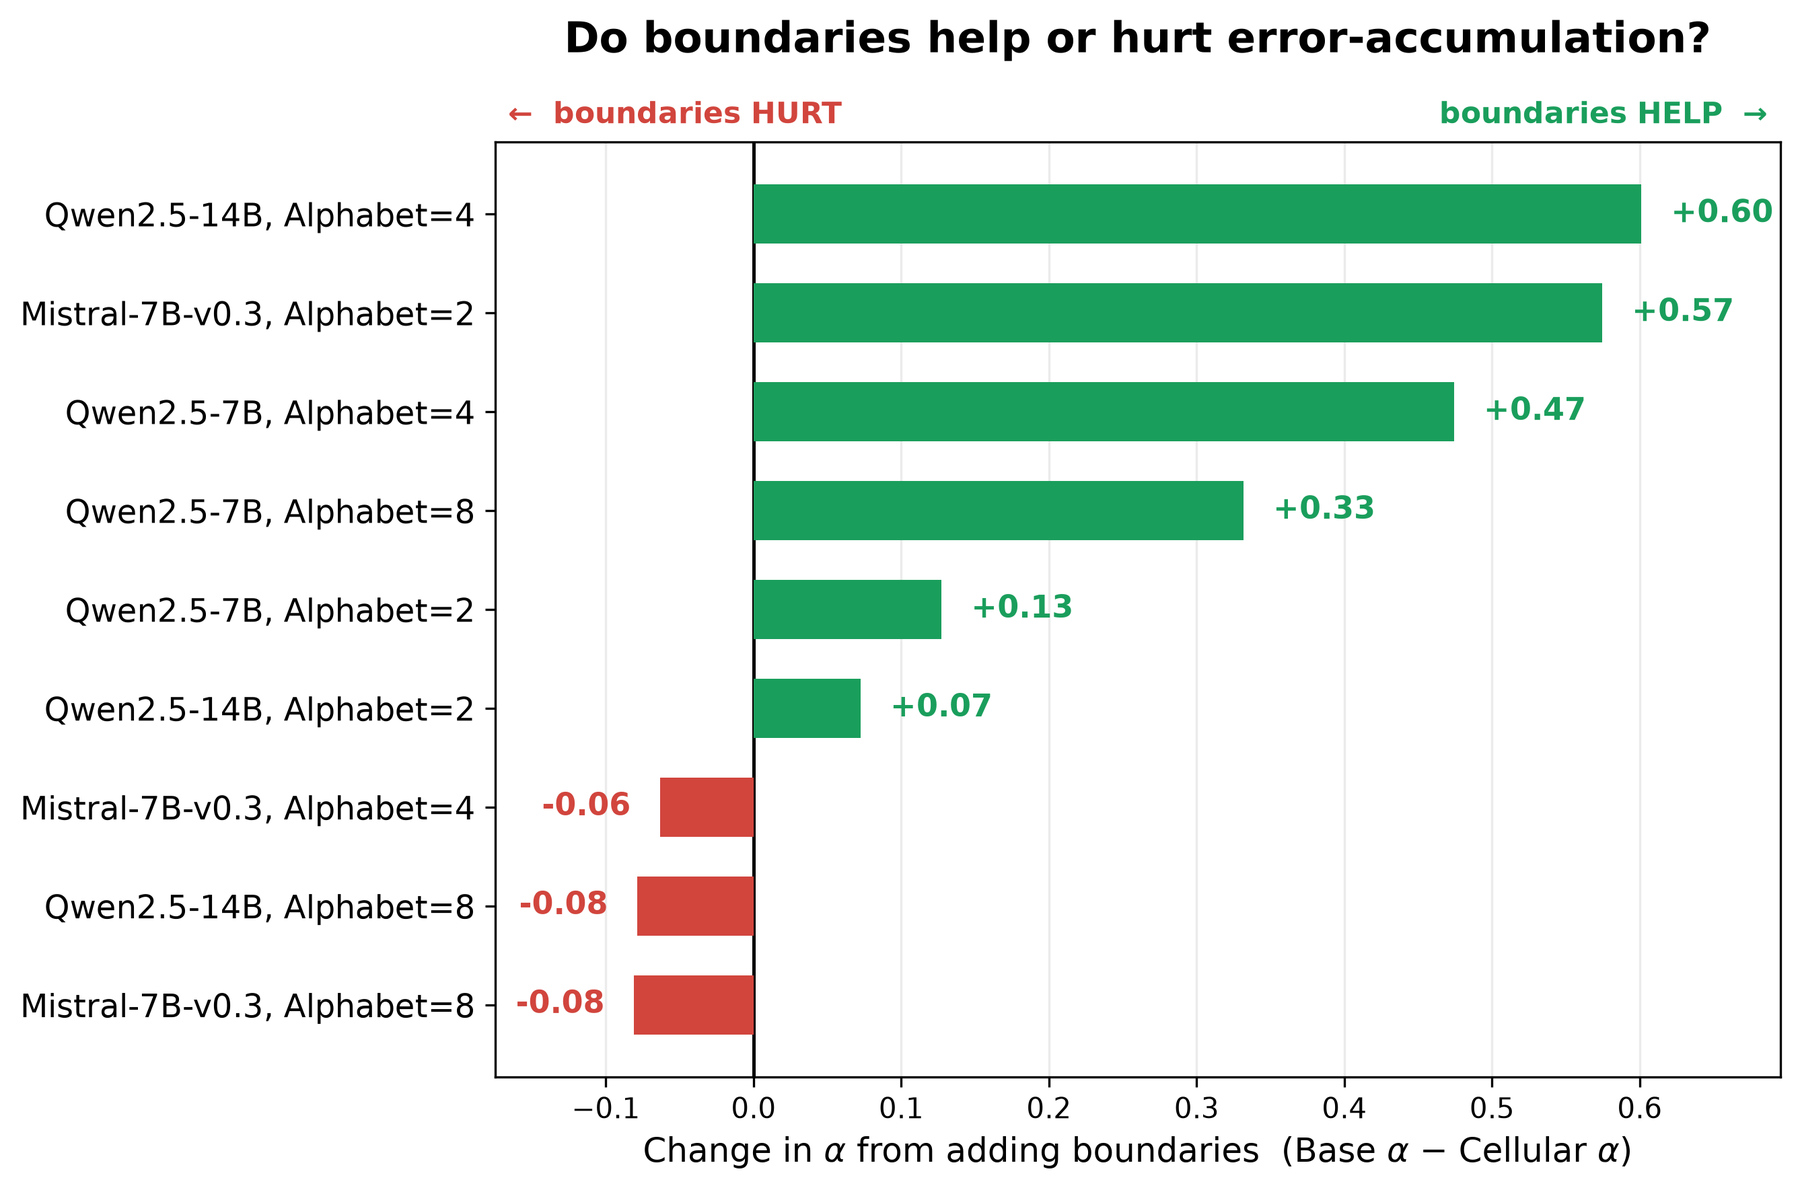
\includegraphics[width=0.85\textwidth]{figures/fig1.png}
  \caption{Every tested (model, alphabet size) combination, sorted by effect size. Each bar is Base $\alpha$ $-$ mean Cellular $\alpha$ (averaged across every boundary density where the SK fit converged); green means boundaries lowered $\alpha$, red means they raised it.}
  \label{fig:fig1}
\end{figure}

Six of nine (model, alphabet) combinations show boundaries reducing $\alpha$; three show the opposite. The split is not random: \textbf{every alphabet=2 combination is green, in all three models}, and two of the three are among the largest effects observed anywhere in this study (Qwen2.5-14B: Base $\alpha = 1.654 \rightarrow$ Cellular $1.053$; Mistral-7B: $1.781 \rightarrow 1.206$). The three combinations where boundaries \emph{increase} $\alpha$ --- Qwen2.5-14B at alphabet=8, and Mistral-7B at both alphabet=4 and alphabet=8 --- are all harder variants of the task.

The honest version of the claim is therefore scoped, not universal: \textbf{structural boundaries substantially and consistently reduce error-accumulation on the simplest version of this task, across model scale and architecture family. On harder variants, the effect is inconsistent, and in a third of the harder cases it reverses.} We are not aware of a principled reason to expect the reversal cases specifically (Qwen-14B/A8, Mistral/A4, Mistral/A8) rather than some other subset, and treat this as an open question rather than force a post-hoc explanation onto it.

\begin{figure}[htbp]
  \centering
  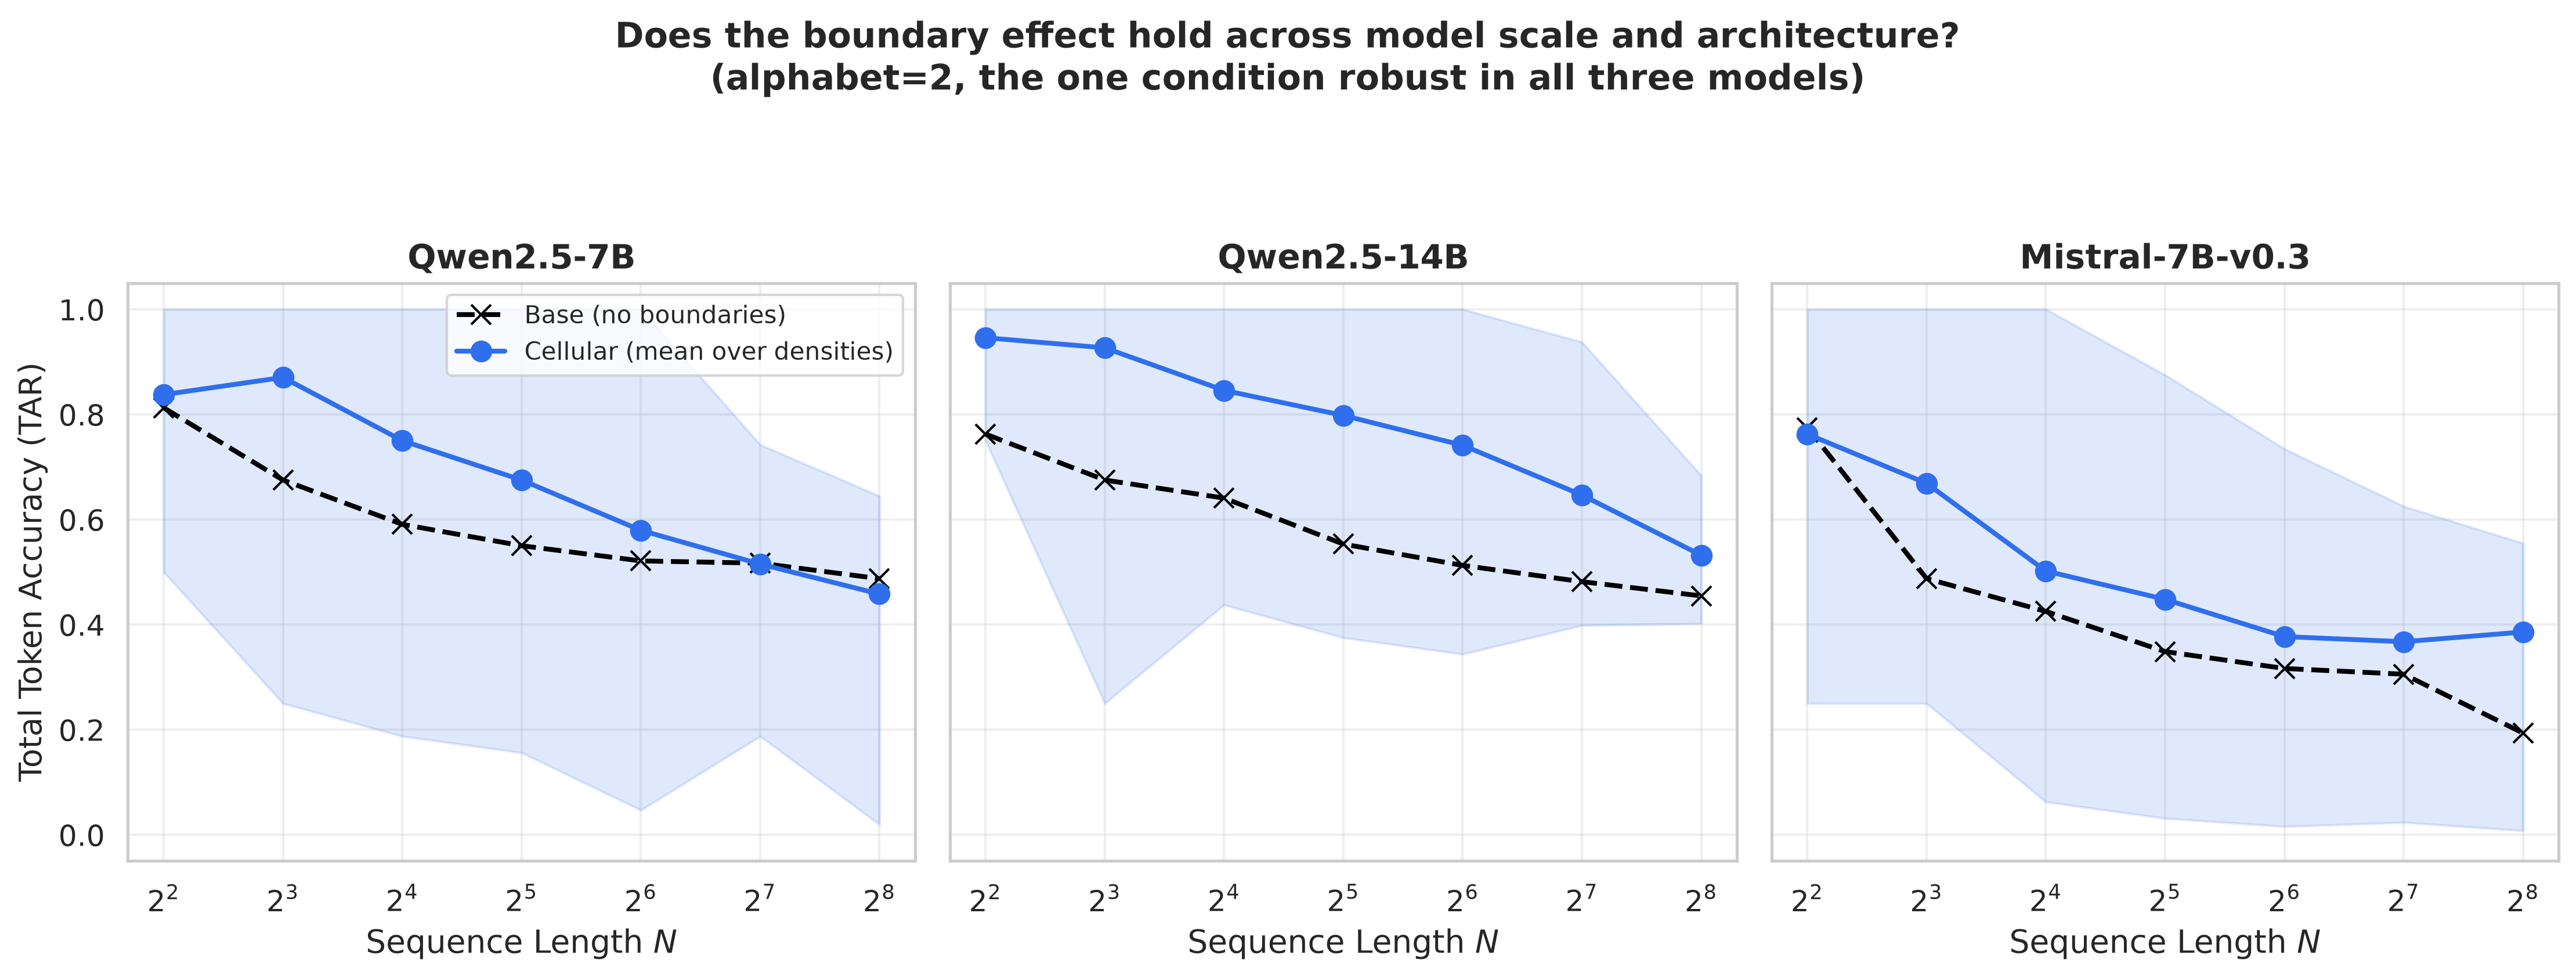
\includegraphics[width=\textwidth]{figures/fig1B.png}
  \caption{TAR vs.\ sequence length, alphabet=2 only, one panel per model. Dashed = Base; solid = Cellular (mean across tested densities; band = full range across densities).}
  \label{fig:fig1B}
\end{figure}

Restricting to the one condition established as robust in Figure~\ref{fig:fig1}, the raw-accuracy picture agrees: Cellular exceeds Base in 18 of 21 (model $\times$ length) combinations. Qwen2.5-14B shows the strongest, most consistent separation, holding at every length out to $N=256$ (0.532 vs.\ 0.454). Mistral-7B shows a narrower but real gap from $N=8$ through $N=256$. Qwen2.5-7B tracks the same pattern through $N=64$, then the two curves converge and cross slightly negative at $N=128$ and $N=256$ --- the one soft spot in an otherwise consistent three-model result.

\subsection{The underlying scaling behavior}

\begin{figure}[htbp]
  \centering
  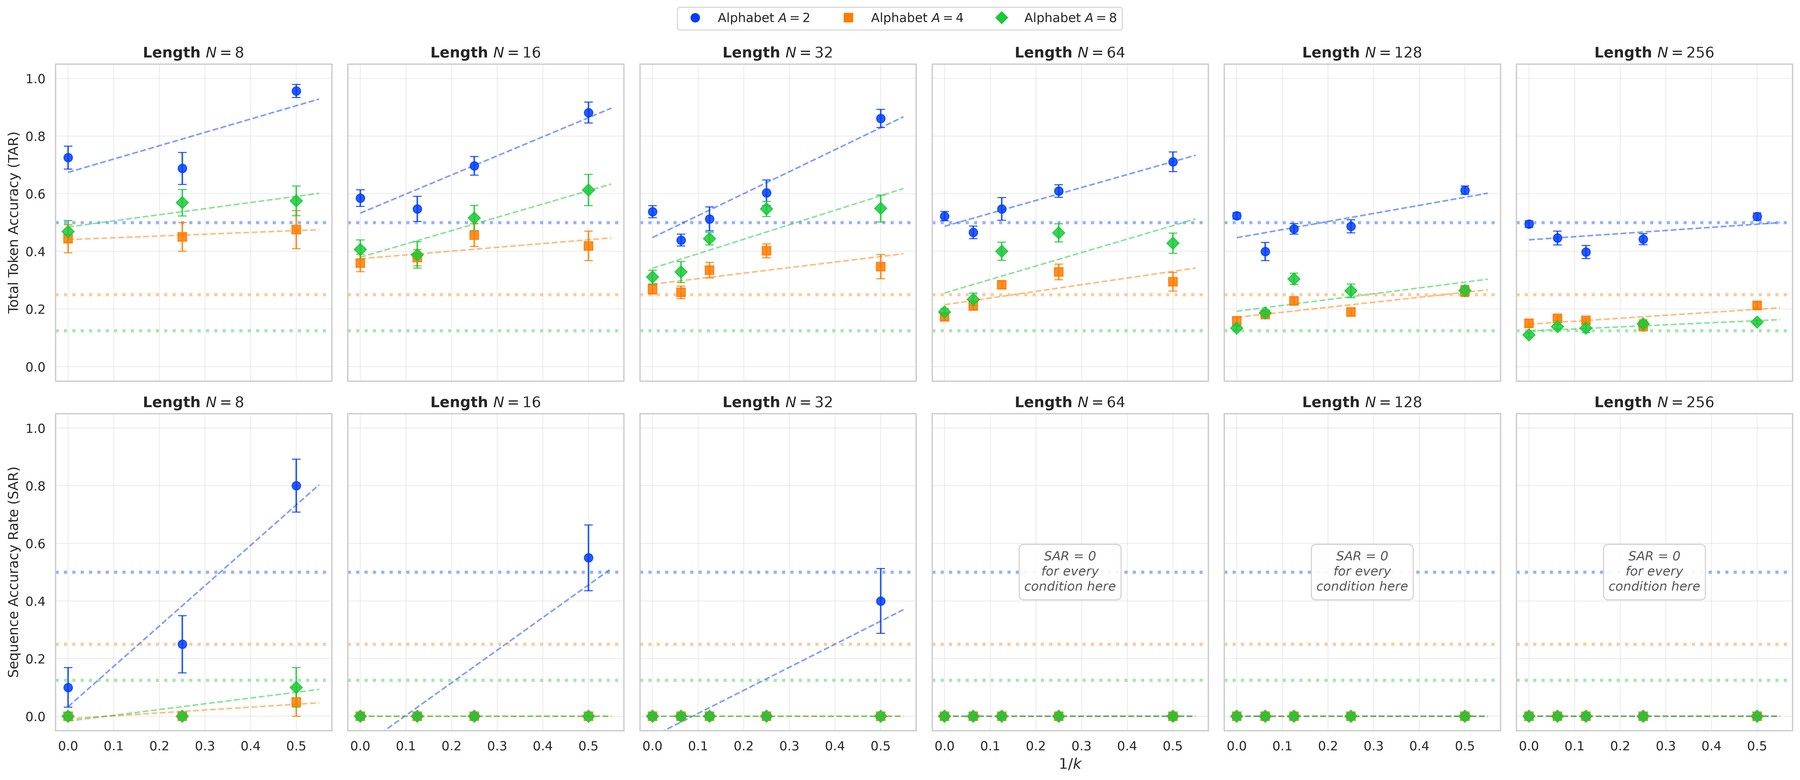
\includegraphics[width=\textwidth]{figures/fig2.png}
  \caption{TAR (top) and SAR (bottom) vs.\ boundary density, faceted by sequence length, Qwen2.5-7B, alphabet $\in \{2, 4, 8\}$. Error bars are SEM across 20 trials.}
  \label{fig:fig2}
\end{figure}

At every tested length, TAR climbs as boundary density increases, and the size of that improvement is largest exactly where it matters most --- at $N \geq 64$, where the Base condition has already sunk toward chance. SAR tells a starker story: it is already pinned near zero for every condition by $N = 32$, and \emph{exactly} zero for every alphabet at every density from $N = 64$ onward (annotated directly on the affected panels, since all three alphabets' markers coincide at the same point and would otherwise look like missing data rather than a genuine unanimous collapse). The practical reading: getting a long sequence \emph{completely} right in one shot is out of reach regardless of boundaries well before the softer, partial-credit metric gives up --- boundaries buy back partial accuracy long after the all-or-nothing metric already has none left to give.

\subsection{Do boundary tokens become attention sinks?}
\label{sec:attention-sinks}

\begin{figure}[htbp]
  \centering
  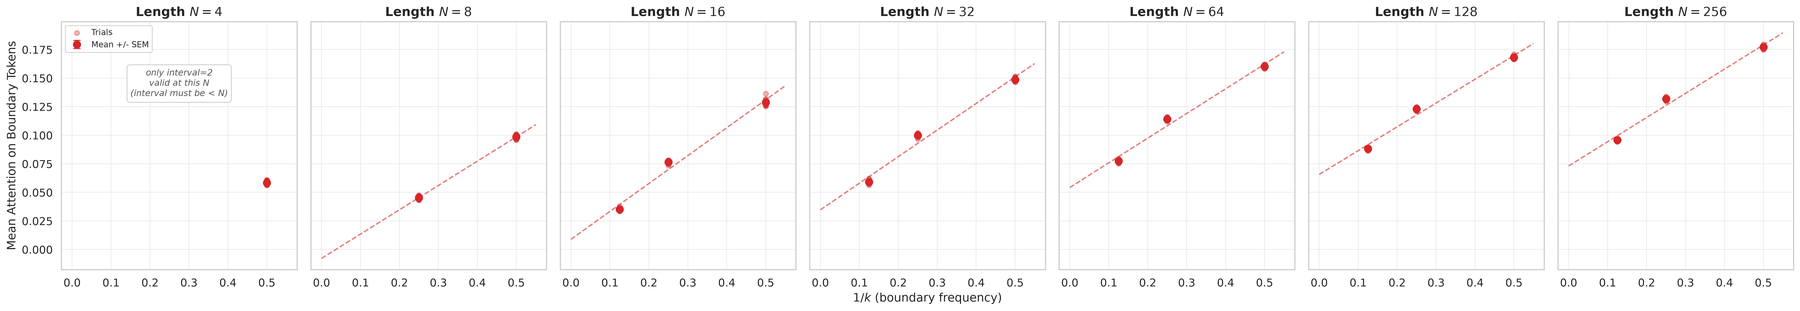
\includegraphics[width=\textwidth]{figures/fig3.png}
  \caption{Mean attention mass landing on boundary tokens vs.\ density, faceted by length, full 20-trial statistical sweep (Qwen2.5-7B).}
  \label{fig:fig3}
\end{figure}

This is the most statistically decisive result in the study: attention mass on boundary tokens rises with density at \emph{every} tested length, with $R^2 \geq 0.98$ in every panel. It is not, however, a length-independent constant --- at the densest tested setting, boundary attention mass climbs from 0.058 at $N=4$ to 0.177 at $N=256$, essentially tripling. What does level off is the \emph{rate} of that growth: the increase from $N=4$ to $N=64$ (0.058 $\rightarrow$ 0.160) dwarfs the increase from $N=64$ to $N=256$ (0.160 $\rightarrow$ 0.177). Boundary tokens become a steadily more important attention target as sequences lengthen, with that importance still rising, just much more slowly, out to the longest lengths tested.

\subsection{Error containment: does the model recover faster after a boundary?}
\label{sec:error-containment}

\begin{figure}[htbp]
  \centering
  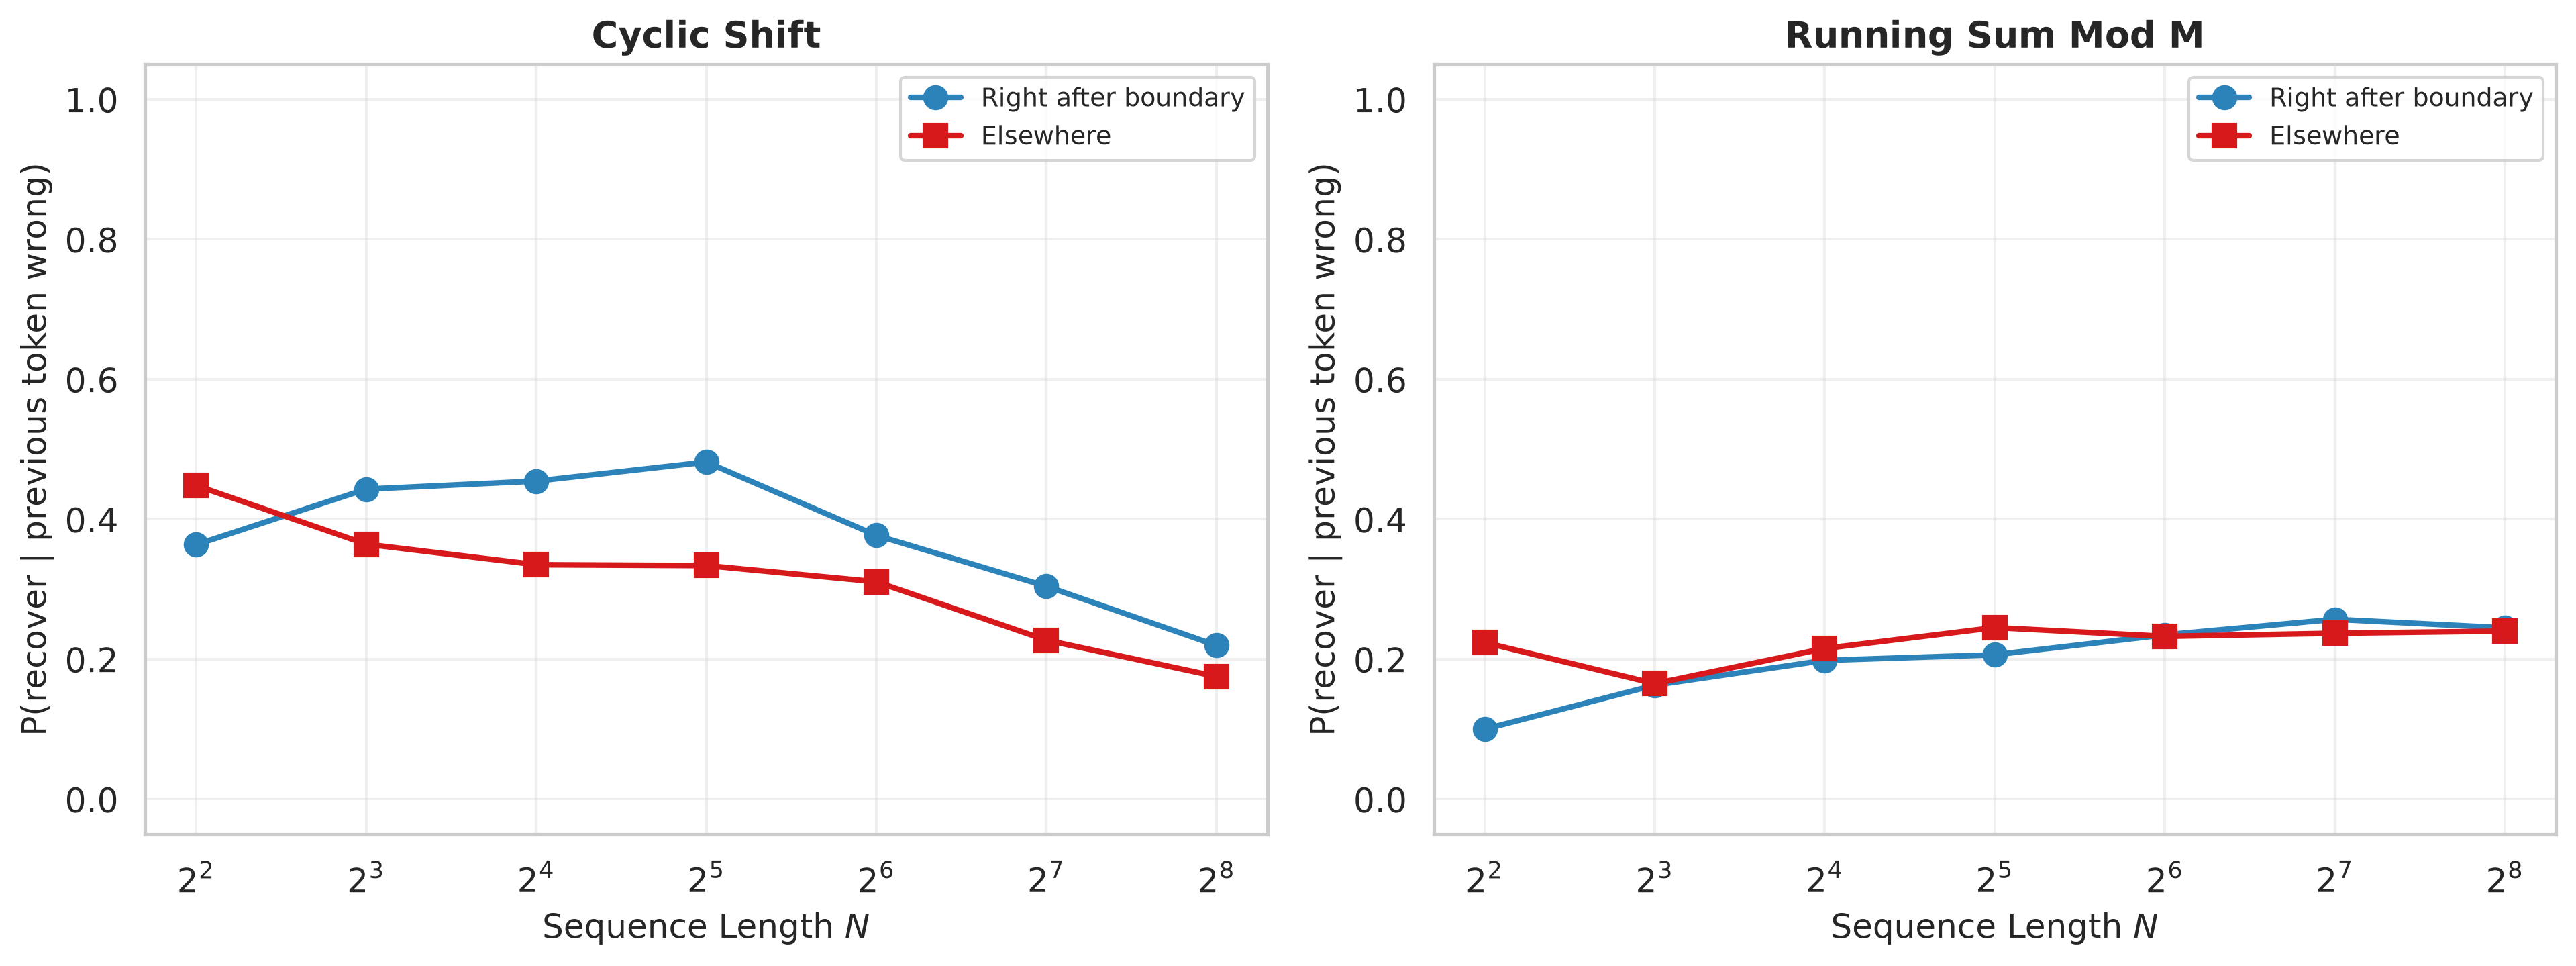
\includegraphics[width=\textwidth]{figures/fig4.png}
  \caption{P(next character correct $\mid$ previous character wrong), split by whether a boundary token was just crossed. Left: cyclic shift. Right: running-sum-mod-$M$.}
  \label{fig:fig4}
\end{figure}

On cyclic shift, recovery immediately after a boundary is measurably and consistently higher than recovery elsewhere, from $N=8$ through $N=256$ --- direct behavioral evidence that boundaries help contain a mistake rather than let it propagate. On running-sum-mod-$M$, no such separation appears at any length; the two curves track each other closely throughout. The most likely explanation is structural: running-sum's correct output at any position depends on the literal cumulative sum of everything before it, so there is no purely local error for a boundary to contain --- a wrong digit corrupts the running state itself, and a marker cannot undo that. This distinction --- does boundary-adjacency help recovery --- turns out to predict which tasks benefit from the intervention at all (Section~\ref{sec:addition}).

\subsection{What about the boundary actually matters?}

\begin{figure}[htbp]
  \centering
  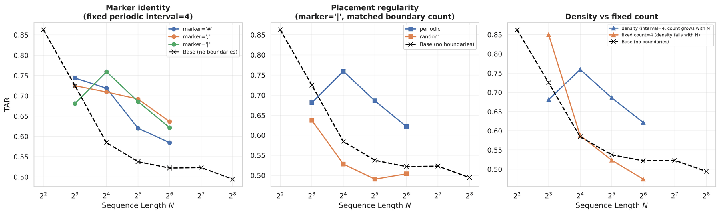
\includegraphics[width=\textwidth]{figures/fig5.png}
  \caption{Three ablations, alphabet=2, all against the same Base reference (TAR at $N=8/16/32/64$: 0.725 / 0.584 / 0.538 / 0.522).}
  \label{fig:fig5}
\end{figure}

\emph{Marker identity} (left panel; \texttt{|} vs.\ \texttt{;} vs.\ \texttt{\#}, fixed periodic interval): all three markers clear Base by a wide margin at every length and show no consistent ranking among themselves (each is briefly ``best'' at some length) --- the symbol's identity or meaning does not matter, provided it is used consistently.

\emph{Placement regularity} (middle panel; periodic vs.\ randomly-scattered, matched total marker count): the sharpest result in this ablation set. Periodic placement stays clearly above Base at every length from $N=16$ on (0.759 vs.\ 0.584 at $N=16$, a 17.5-point gap). Randomly-scattered markers with the \emph{identical total count} fall \emph{below} Base at $N=16$ and $N=32$ (0.528 and 0.491, vs.\ 0.584 and 0.538) and only catch back up to roughly even by $N=64$. Regularity of placement, not mere presence of markers, is doing the work.

\emph{Density vs.\ raw count} (right panel; constant interval, so marker count scales with $N$, vs.\ a fixed count of 4 markers regardless of $N$): a fixed count of 4 markers is very dense at $N=8$ (one marker per 2 characters) and correspondingly strong there (TAR 0.850, beating even Base's 0.725) --- but by $N=64$ those same 4 markers are spread so thin (one per 16 characters) that TAR falls to 0.474, \emph{below} Base with no markers at all (0.522). The density-preserving condition, which keeps adding markers as $N$ grows, stays at 0.622 at $N=64$. Density, not a one-time dose of structure, is the operative variable.

\textbf{Does the marker need to be a single unusual character?} The three markers above (\texttt{|}, \texttt{;}, \texttt{\#}) are all single, visually distinctive characters. We additionally tested two multi-character markers (\texttt{||}, \texttt{<|>}) and two naturally-occurring tokens that already appear in ordinary text (newline, comma), fixed interval=4, same seeds as the single-character ablation grid above.

\begin{figure}[htbp]
  \centering
  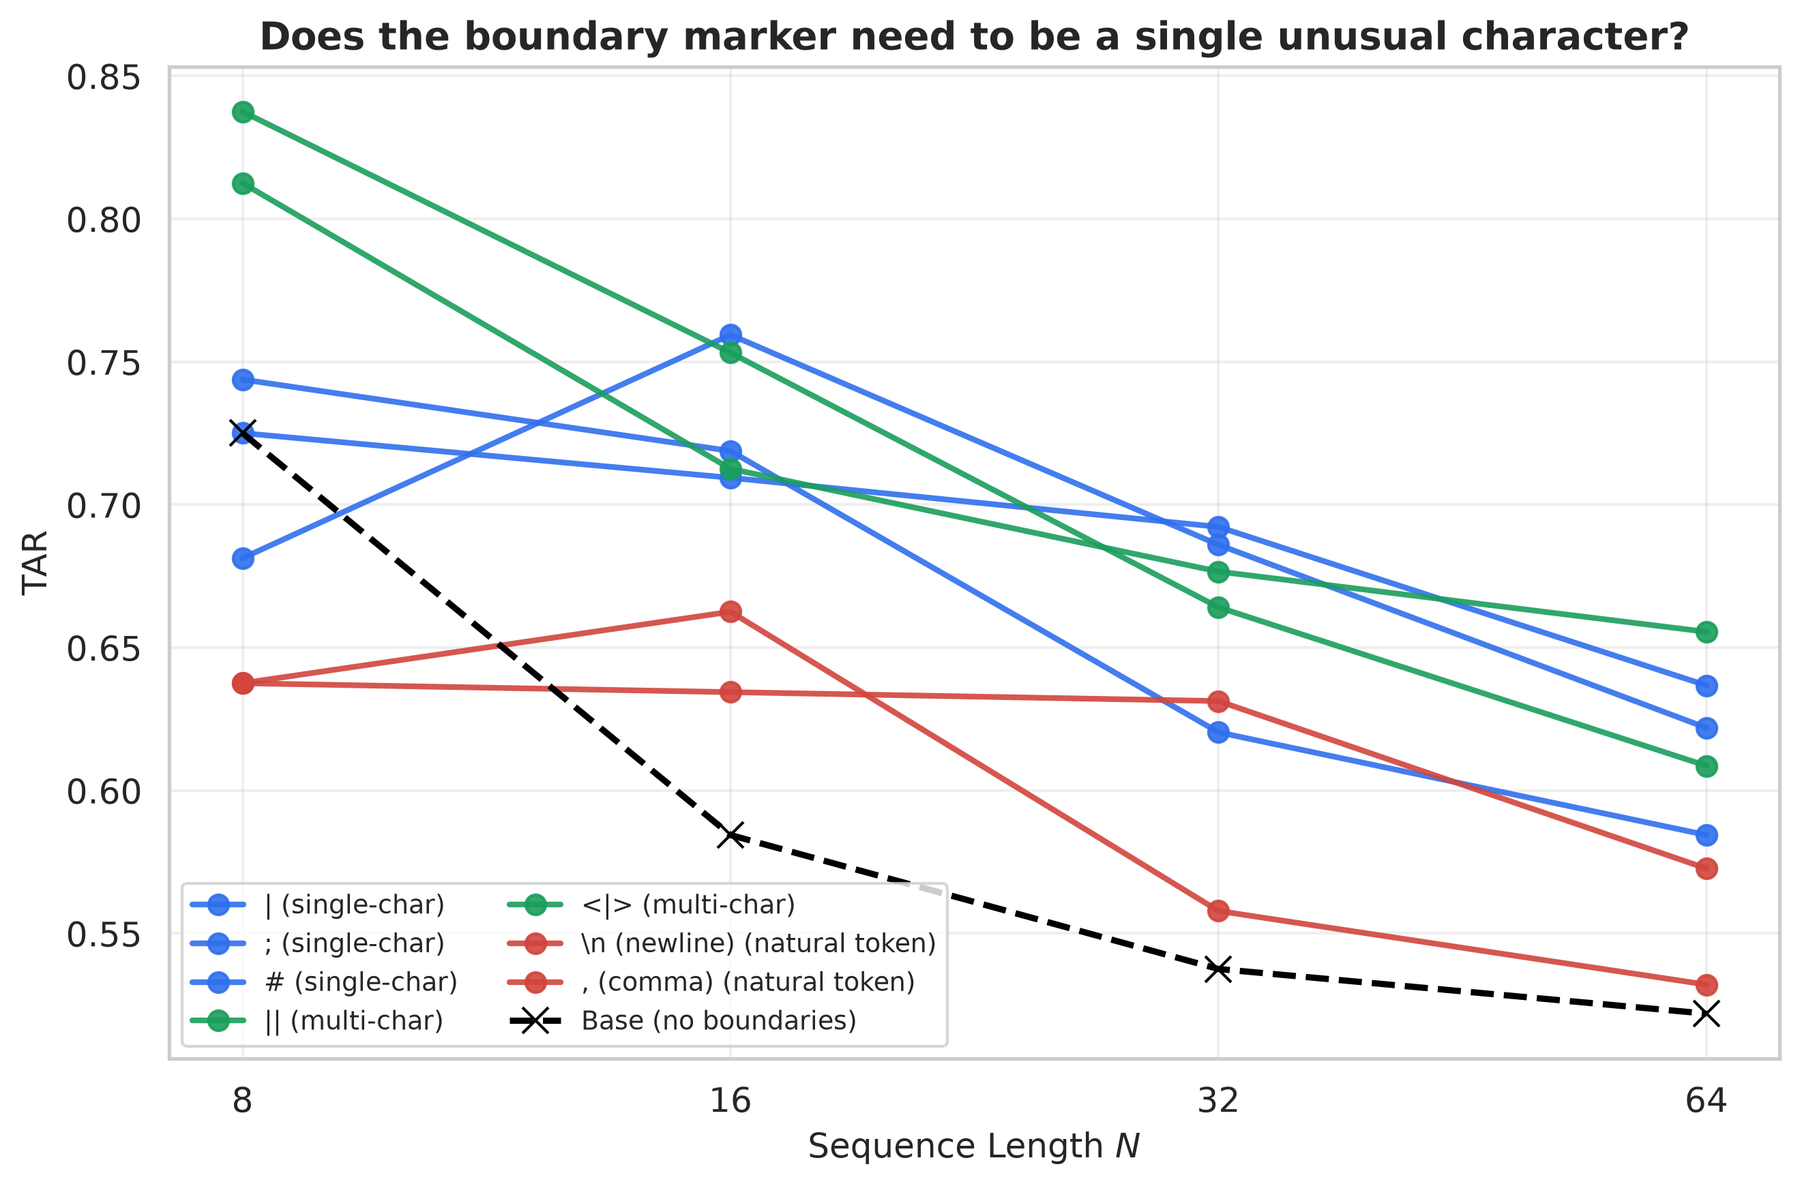
\includegraphics[width=\textwidth]{figures/fig18.png}
  \caption{TAR vs.\ sequence length for seven marker variants (single-character, multi-character, and natural-token), alphabet=2, interval=4, Qwen2.5-7B, against the same Base reference.}
  \label{fig:fig18}
\end{figure}

Multi-character markers are, if anything, among the strongest performers: \texttt{||} is the single best-performing marker at $N=8$ (TAR 0.838, vs.\ Base's 0.725) and \texttt{<|>} is the best at $N=64$ (0.656, vs.\ Base's 0.522) --- extending the marker from one character to two or three does not degrade the effect. The natural-token markers (newline, comma) tell a different story, and the one genuine exception to this whole ablation set appears here: at $N=8$, \emph{both} natural tokens actually score \emph{below} Base (0.638 vs.\ 0.725) --- the only condition anywhere in Figure~\ref{fig:fig5} or Figure~\ref{fig:fig18} where a boundary marker underperforms having no boundaries at all. From $N=16$ on, both natural tokens do clear Base, but by a visibly narrower margin than any of the five deliberately-chosen markers, and for comma specifically that margin shrinks to nearly nothing by $N=64$ (0.532 vs.\ Base's 0.522, a gap of 0.010, against gaps of 0.06--0.13 for every deliberately-chosen marker at the same length). One scoring subtlety is worth flagging explicitly: because the standard response-cleanup step truncates a model's output at its first newline (to strip trailing ``Explanation'' chatter), using \texttt{"\textbackslash n"} itself as the boundary marker required disabling that truncation specifically for this condition, since otherwise the model's own echoed boundary would truncate its answer before scoring. The overall picture is consistent with marker \emph{distinctiveness} mattering, not merely presence: a marker's identity is fungible among symbols chosen specifically not to occur in the task's normal vocabulary (any of \texttt{|}, \texttt{;}, \texttt{\#}, \texttt{||}, \texttt{<|>} work comparably well), but a token the model already sees constantly in ordinary text is a measurably weaker structural signal, and can even actively hurt at short lengths.

\textbf{A tokenization caveat.} Marker length in characters is not the same as marker length in tokens, and this matters for how the \texttt{<|>} result above should be read. Tokenizing each marker with Qwen2.5-7B-Instruct's own tokenizer, in the actual context these experiments use (alphabet=2, $N=16$, interval=4, 3 boundaries inserted): \texttt{|}, \texttt{;}, \texttt{\#}, the newline, and the comma each produce an 11-token encoding of the full input string, and --- because of BPE merging --- so does \texttt{||}, despite being two characters. \texttt{<|>}, however, encodes as \texttt{<}, \texttt{|}, \texttt{>} (three separate tokens), producing a 17-token encoding of the identical input for the identical nominal $N$. This means \texttt{||}'s result is a genuinely token-count-matched test of marker length: two characters, still one token, performing comparably to every single-character marker. \texttt{<|>}'s strong performance is not: at matched character-level interval, it injects three times the token-level structural signal per boundary that every other marker in this comparison does, so its result should be read as evidence that \emph{more boundary tokens per checkpoint can help}, not as a clean test of whether marker length itself is what matters. This sweep does not contain a token-count-matched multi-token marker (e.g.\ a two-token symbol used at the same overall token budget as the single-token markers), which would be needed to cleanly separate these two explanations --- flagged here as a concrete gap for follow-up work rather than retroactively reinterpreted from the existing data.

\subsection{A negative result: integer addition}
\label{sec:addition}

\begin{figure}[htbp]
  \centering
  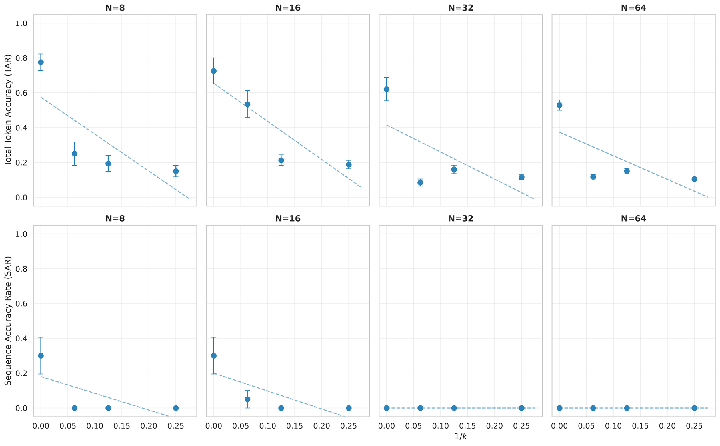
\includegraphics[width=\textwidth]{figures/fig6.png}
  \caption{TAR/SAR vs.\ density, integer addition, Qwen2.5-7B.}
  \label{fig:fig6}
\end{figure}

The direction of the effect reverses completely. At every one of four tested lengths ($N=8, 16, 32, 64$), Base is the \emph{best}-performing condition, and TAR falls further as boundary density increases. SAR is pinned near floor almost everywhere regardless of density, so this task is already difficult in absolute terms --- but boundaries make the partial-credit picture actively worse, not merely neutral. The likely explanation parallels running-sum-mod-$M$ (Section~\ref{sec:error-containment} discussion above): a digit's correct output in addition depends on carry state propagating right-to-left, opposite to left-to-right generation order, so it carries the same genuine long-range dependency. Slicing the sequence into visually separate cells does not just fail to help here --- it appears to actively interfere with tracking that dependency across the boundary. We separately tested whether reversing digit order (so carry direction matches generation direction) rescues the effect; it did not fully do so, and whether letting the model show intermediate step-by-step reasoning (a ``scratchpad'') changes this picture returned an inconclusive result (Section~\ref{sec:discussion}).

\subsection{Is the effect an artifact of one specific prompt?}
\label{sec:prompt-robustness}

\begin{figure}[htbp]
  \centering
  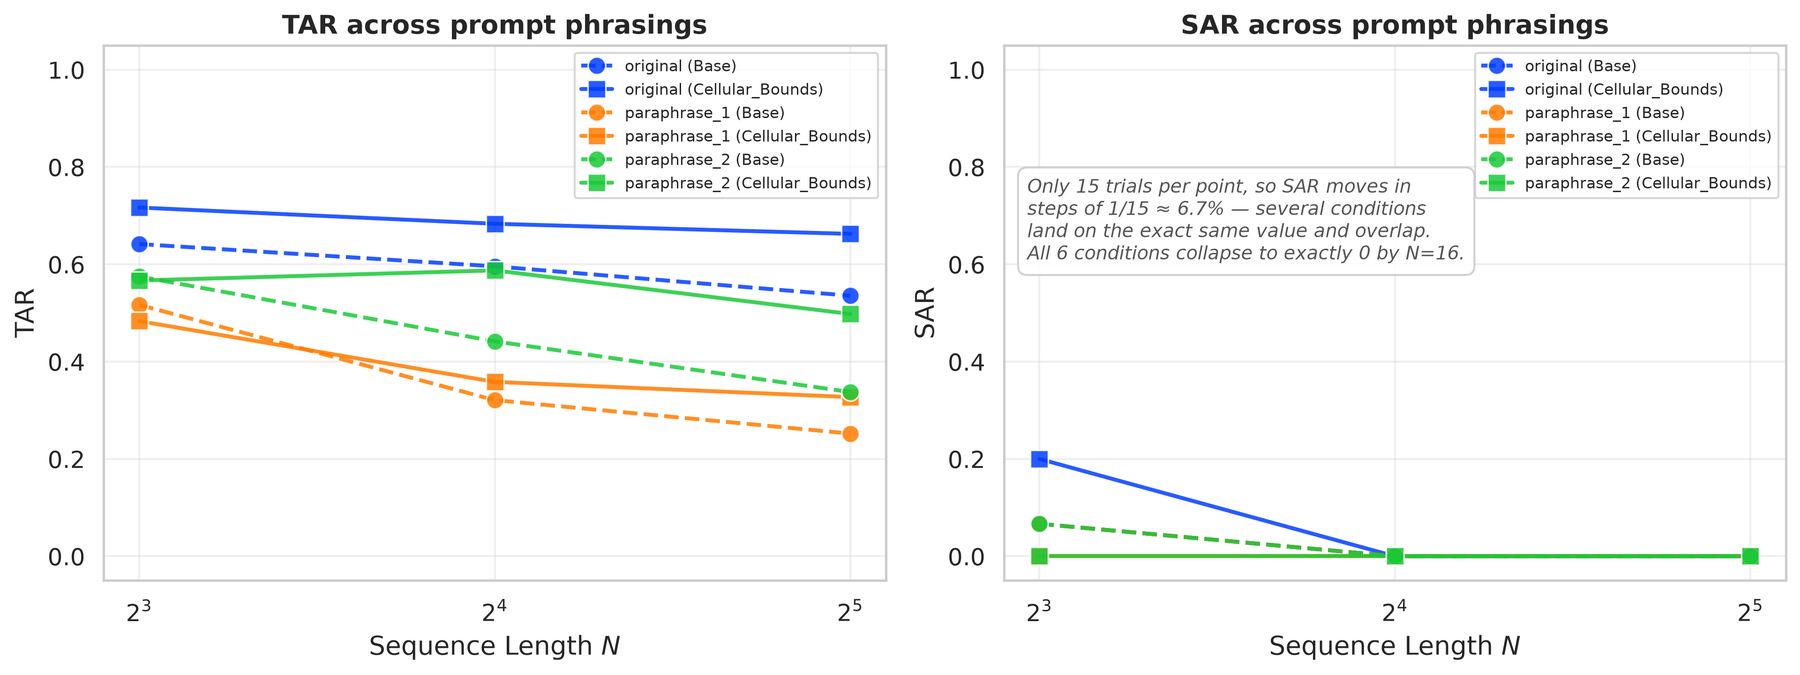
\includegraphics[width=\textwidth]{figures/fig7.png}
  \caption{TAR (left) and SAR (right) vs.\ length, cyclic shift, repeated across three independently-worded instruction templates.}
  \label{fig:fig7}
\end{figure}

Under the original wording, Cellular exceeds Base at all three tested lengths. Both paraphrased templates --- worded quite differently from the original and from each other (formal specification vs.\ casual instruction vs.\ terse cipher notation; see Appendix~\ref{app:prompts} for full prompt text) --- behave almost identically to \emph{each other}, not oppositely: both are essentially tied with Base at the shortest length ($N=8$), then Cellular pulls ahead at $N=16$ and $N=32$ for both, with one paraphrase's $N=32$ gap ($+0.160$) the largest in the whole figure. Across all three templates and lengths, Cellular is ahead in 7 of 9 combinations, behind in the remaining 2 (both by less than 0.03, both at the shortest length only). Wording has some influence on effect size, but the result is not a fragile artifact of one specific script.

\subsection{The chat-template correction, quantified}

\begin{figure}[htbp]
  \centering
  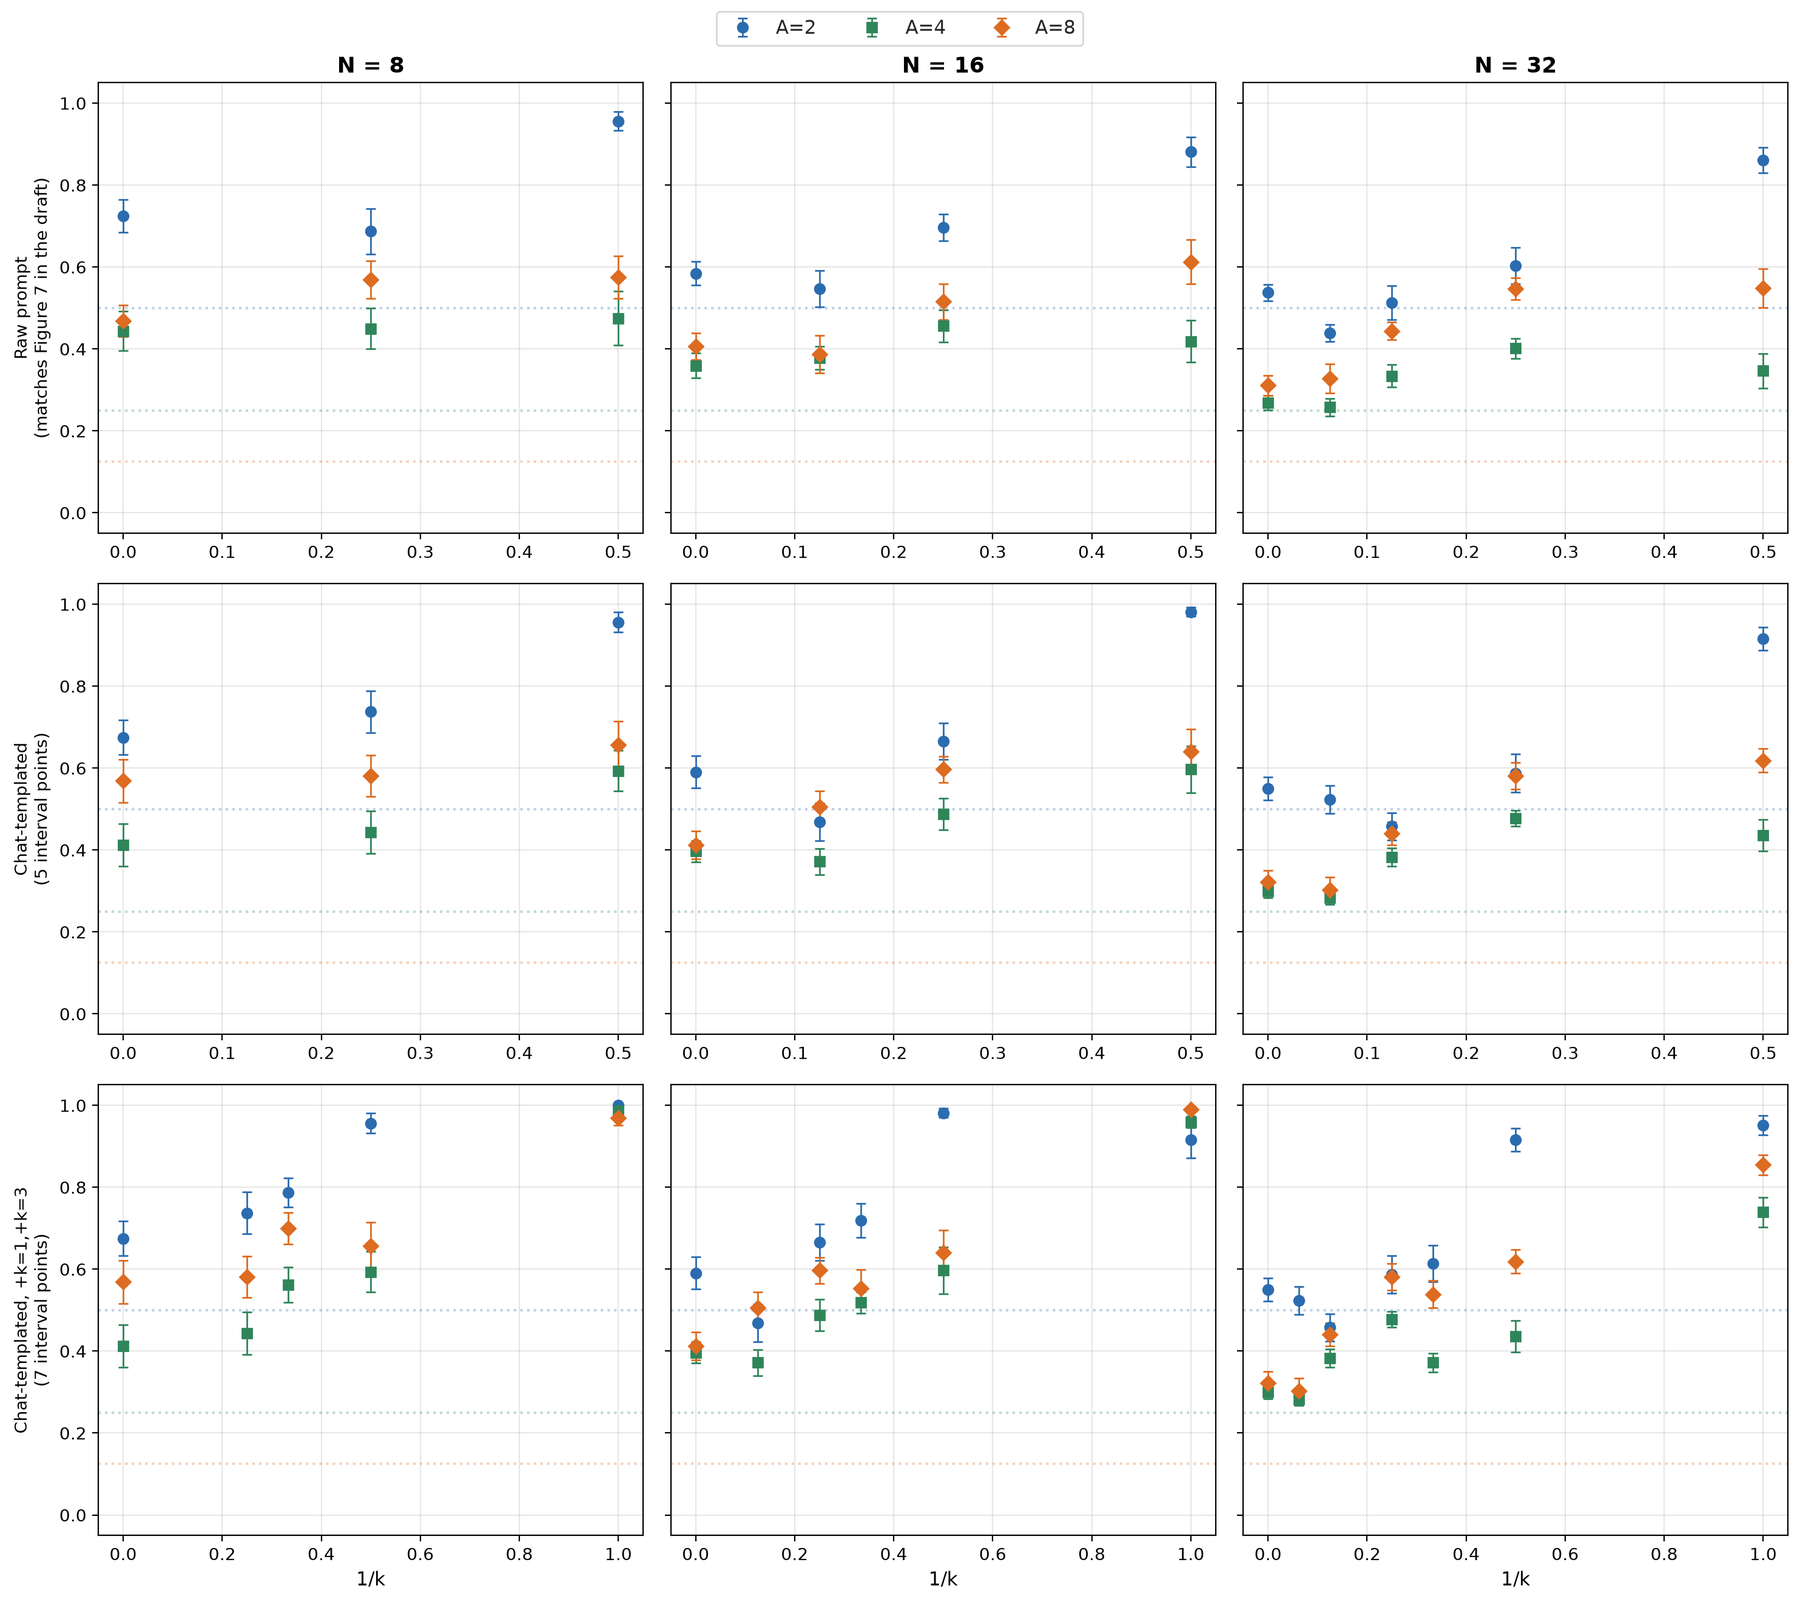
\includegraphics[width=\textwidth]{figures/fig8.png}
  \caption{Same task and data, three prompting methods stacked top to bottom: original raw-text prompting, chat-template-corrected, and chat-template-corrected with an extended density grid.}
  \label{fig:fig8}
\end{figure}

\begin{figure}[htbp]
  \centering
  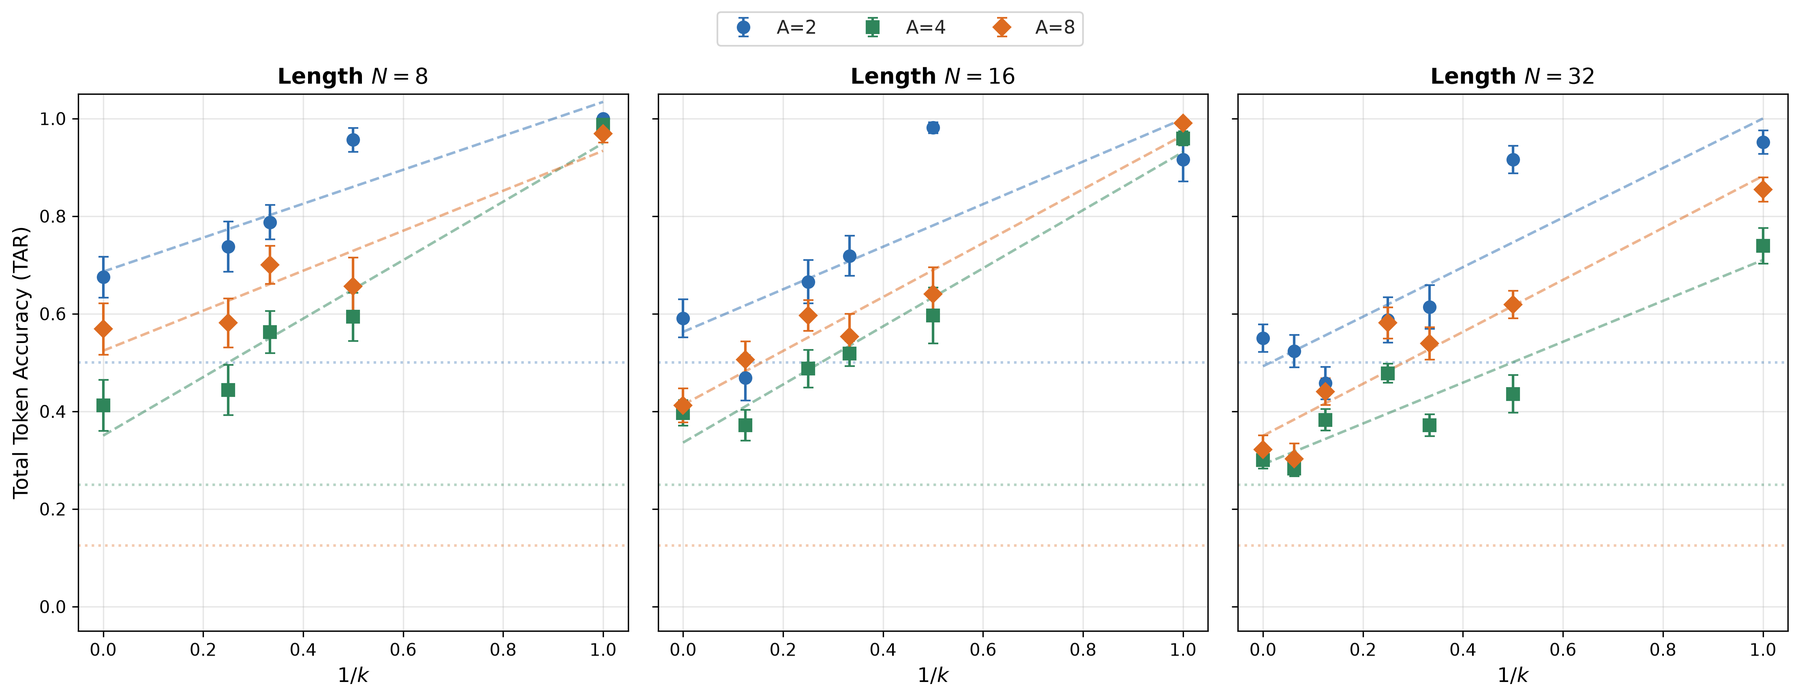
\includegraphics[width=\textwidth]{figures/fig9.png}
  \caption{The finalized scaling law across all seven tested densities ($k = 0, 1, 2, 3, 4, 8, 16$), chat-template-corrected.}
  \label{fig:fig9}
\end{figure}

The 8-symbol alphabet condition is noisy and inconsistent under raw-text prompting, and firms up substantially once the model is prompted in its documented chat format --- direct evidence that prompting an instruction-tuned model outside its trained format does not add noise evenly across conditions, it distorts some conditions more than others. With the density grid extended from 3 points to 7, every alphabet at every tested length traces a clean, consistently upward, near-monotonic curve from sparse to dense boundaries (Figure~\ref{fig:fig9}) --- the single clearest view of the core accuracy result in this study.

\subsection{Mechanistic detail: a single attention head, multi-trial averaged}

\begin{figure}[htbp]
  \centering
  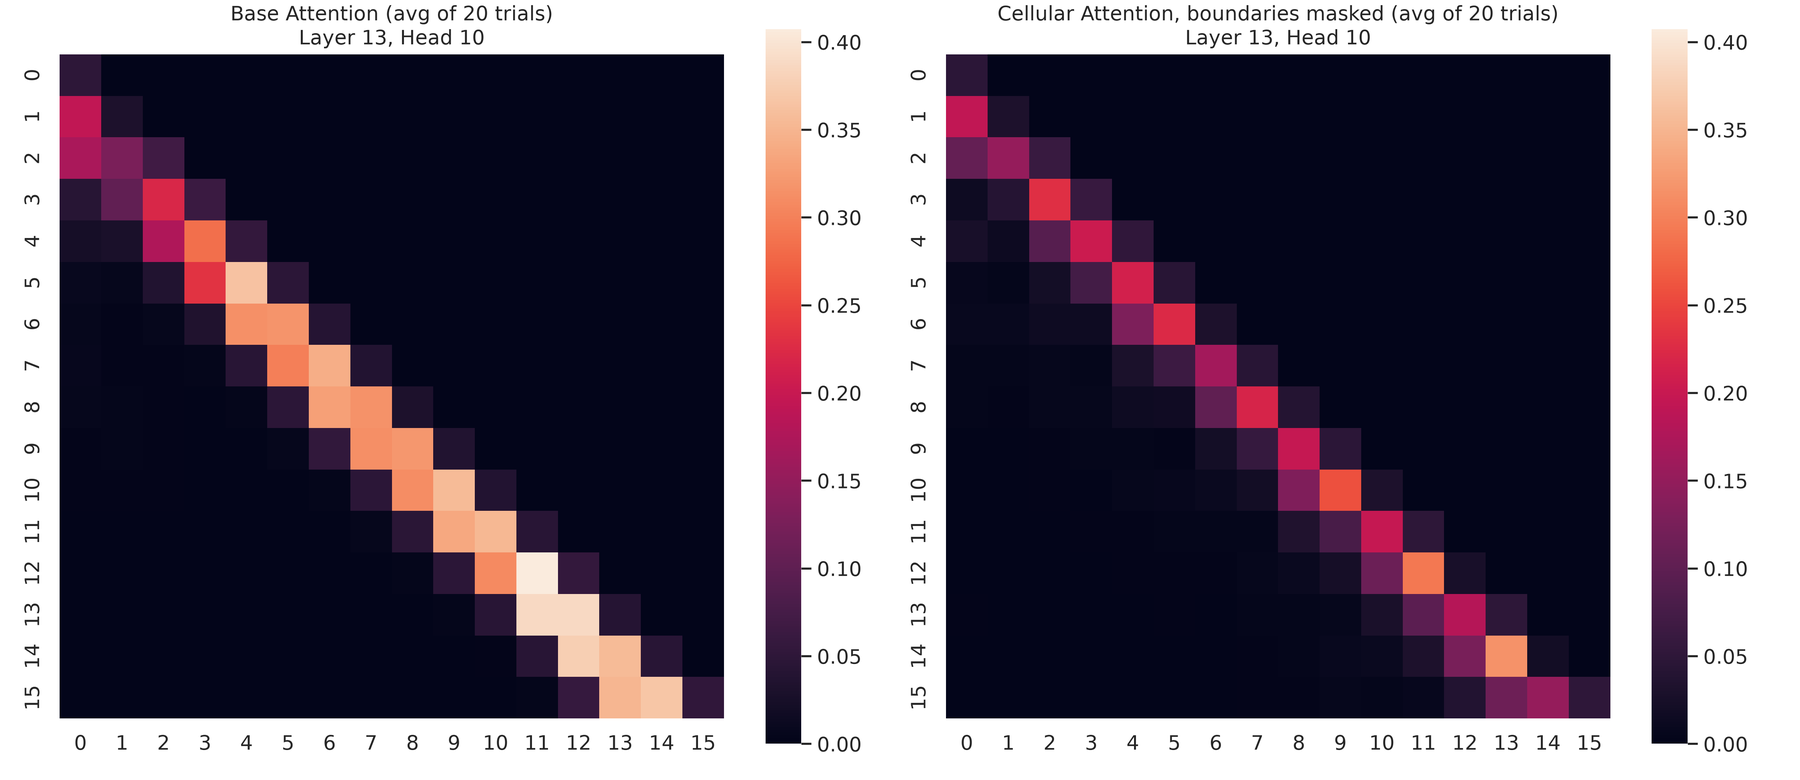
\includegraphics[width=\textwidth]{figures/fig10.png}
  \caption{Layer 13, Head 10 attention, averaged over 20 trials at a fixed configuration (alphabet=2, N=16, k=2); boundary tokens masked out.}
  \label{fig:fig10}
\end{figure}

\begin{figure}[htbp]
  \centering
  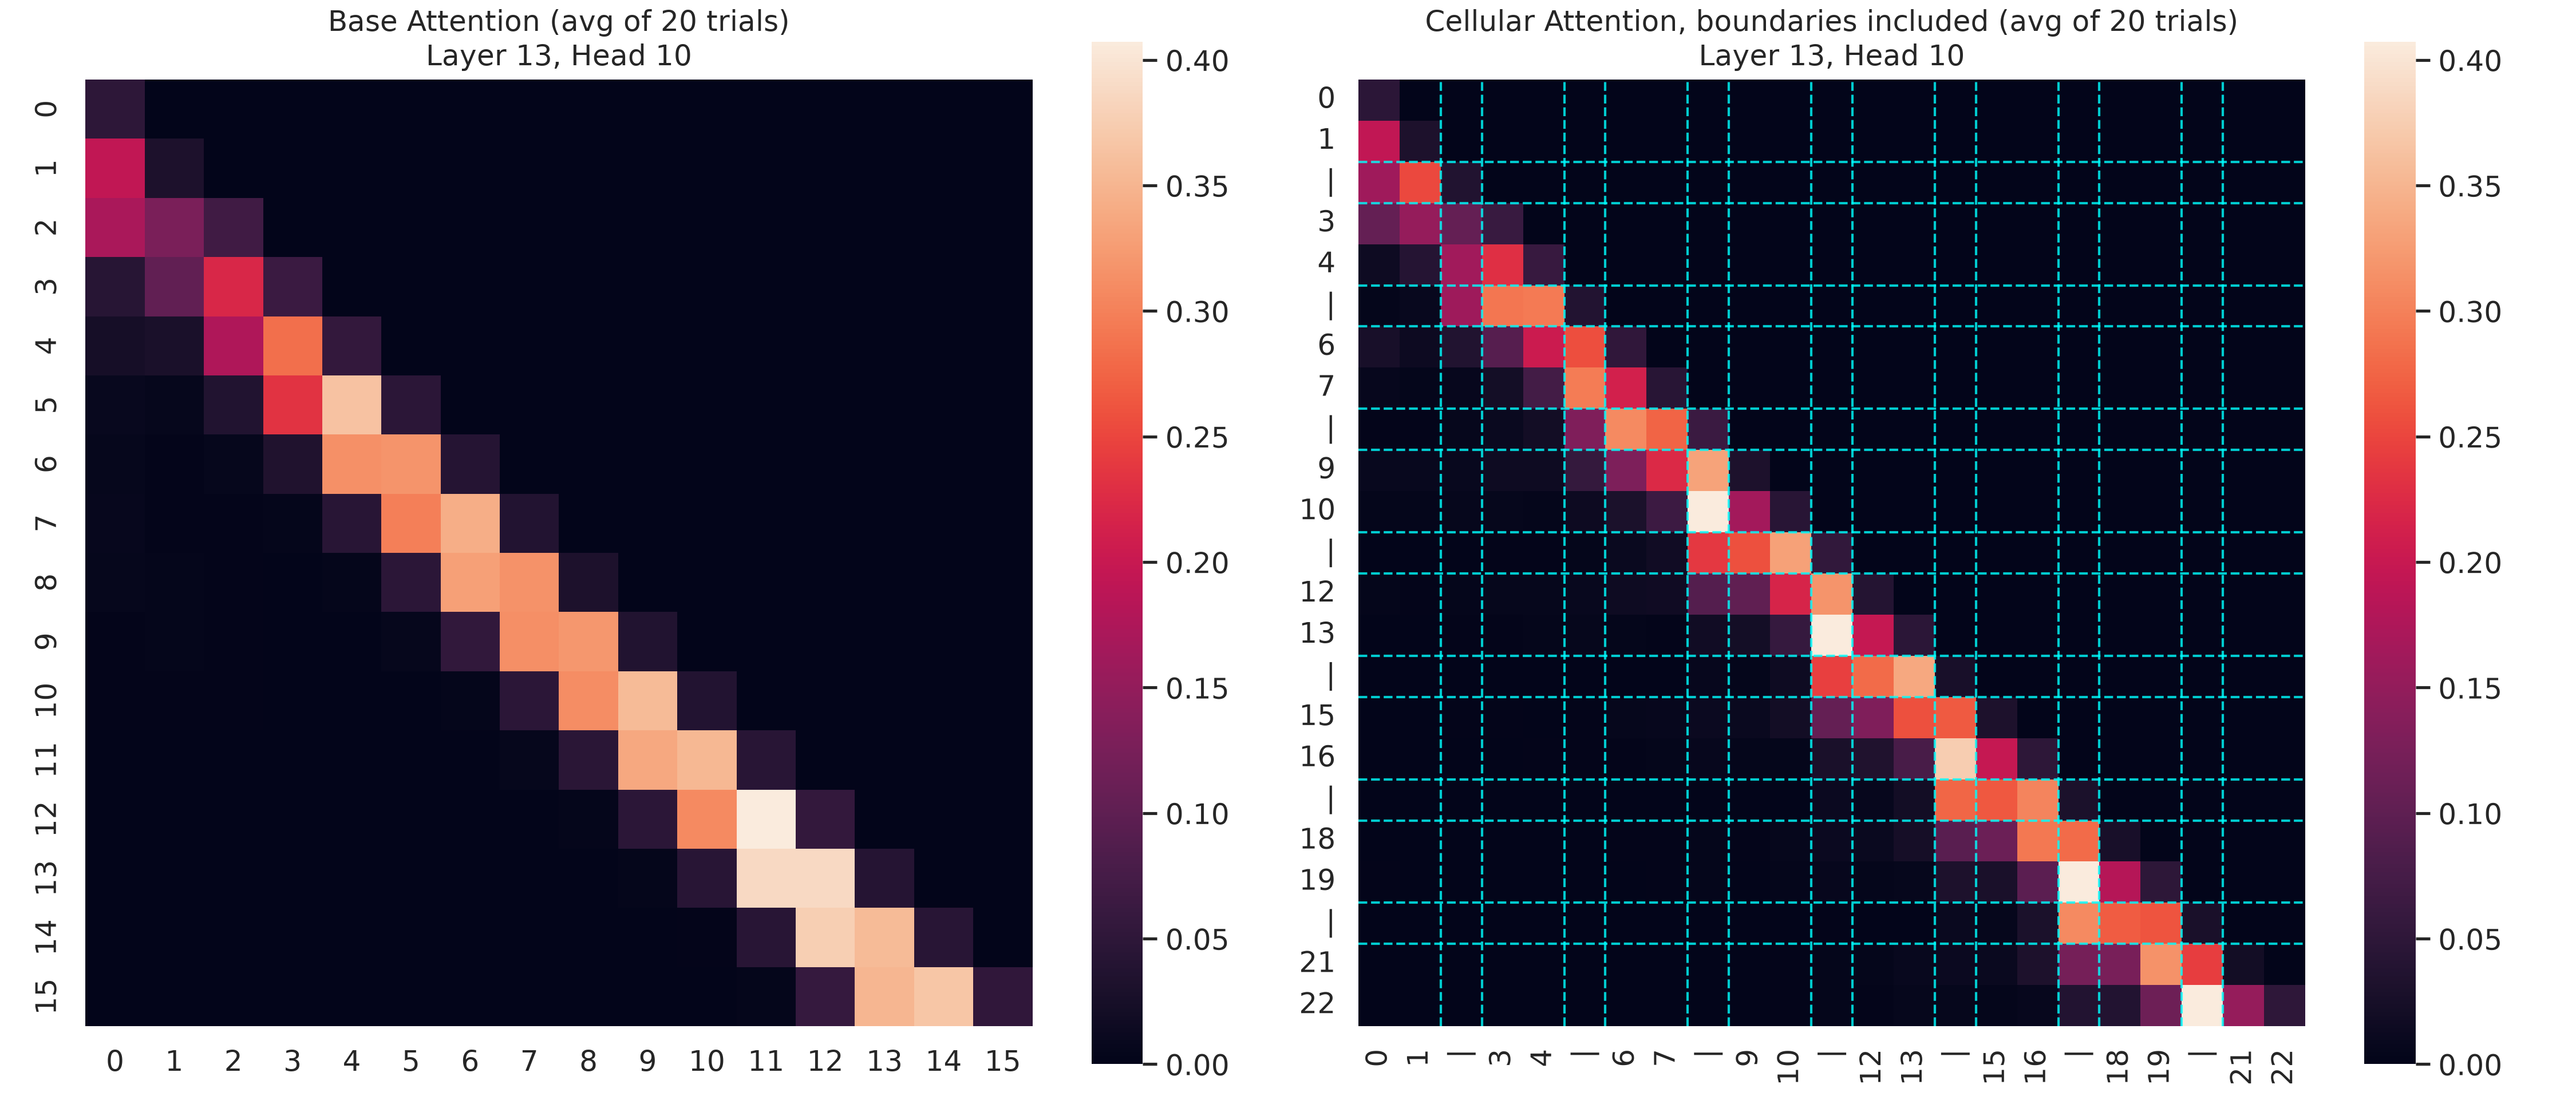
\includegraphics[width=\textwidth]{figures/fig11.png}
  \caption{The same attention pattern as Figure~\ref{fig:fig10}, with boundaries left visible.}
  \label{fig:fig11}
\end{figure}

At the level of a single representative head, Base and Cellular attention look similarly local and diagonal (mean self-attention weight 0.067 in both conditions) --- boundaries do not disrupt the basic letter-to-letter attention habit. Once boundary tokens are left visible (Figure~\ref{fig:fig11}), they visibly pull in extra attention exactly where the diagonal crosses them. Put together with the per-layer breakdown below, this is the clearest single mechanistic picture available: attention stays local within each boundary-delimited cell, and boundary tokens absorb a real, measurable, and --- per Figure~\ref{fig:fig3} --- density-dependent share of attention that a wrong token several cells back has comparatively little pathway left to exploit.

\begin{figure}[htbp]
  \centering
  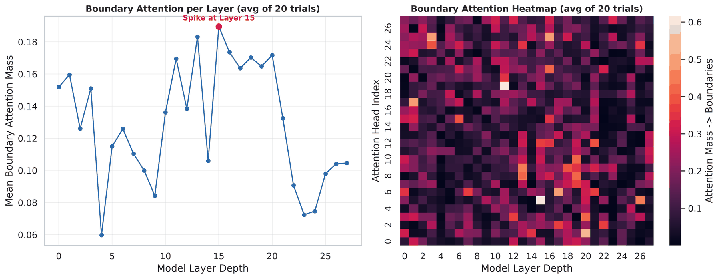
\includegraphics[width=\textwidth]{figures/fig12.png}
  \caption{Boundary-token attention mass by layer (left) and by individual head (right), 20-trial average.}
  \label{fig:fig12}
\end{figure}

Boundary attention peaks mid-network (layer 15, mean 0.190 across heads) but is not a property of whole layers switching on uniformly --- it is concentrated in a scattered subset of individual heads clustered loosely around layers 0--1, 10--11, 15--16, and 18--20. The per-layer average in the left panel is really surfacing where those specific heads happen to cluster, not a layer-wide effect. This matches the full statistical sweep directly: aggregate boundary attention rises monotonically with density (0.071 $\rightarrow$ 0.099 $\rightarrow$ 0.134, sparsest to densest interval tested).

\subsection{Attention entropy: a caught mistake, resolved}
\label{sec:entropy-catch}

\begin{figure}[htbp]
  \centering
  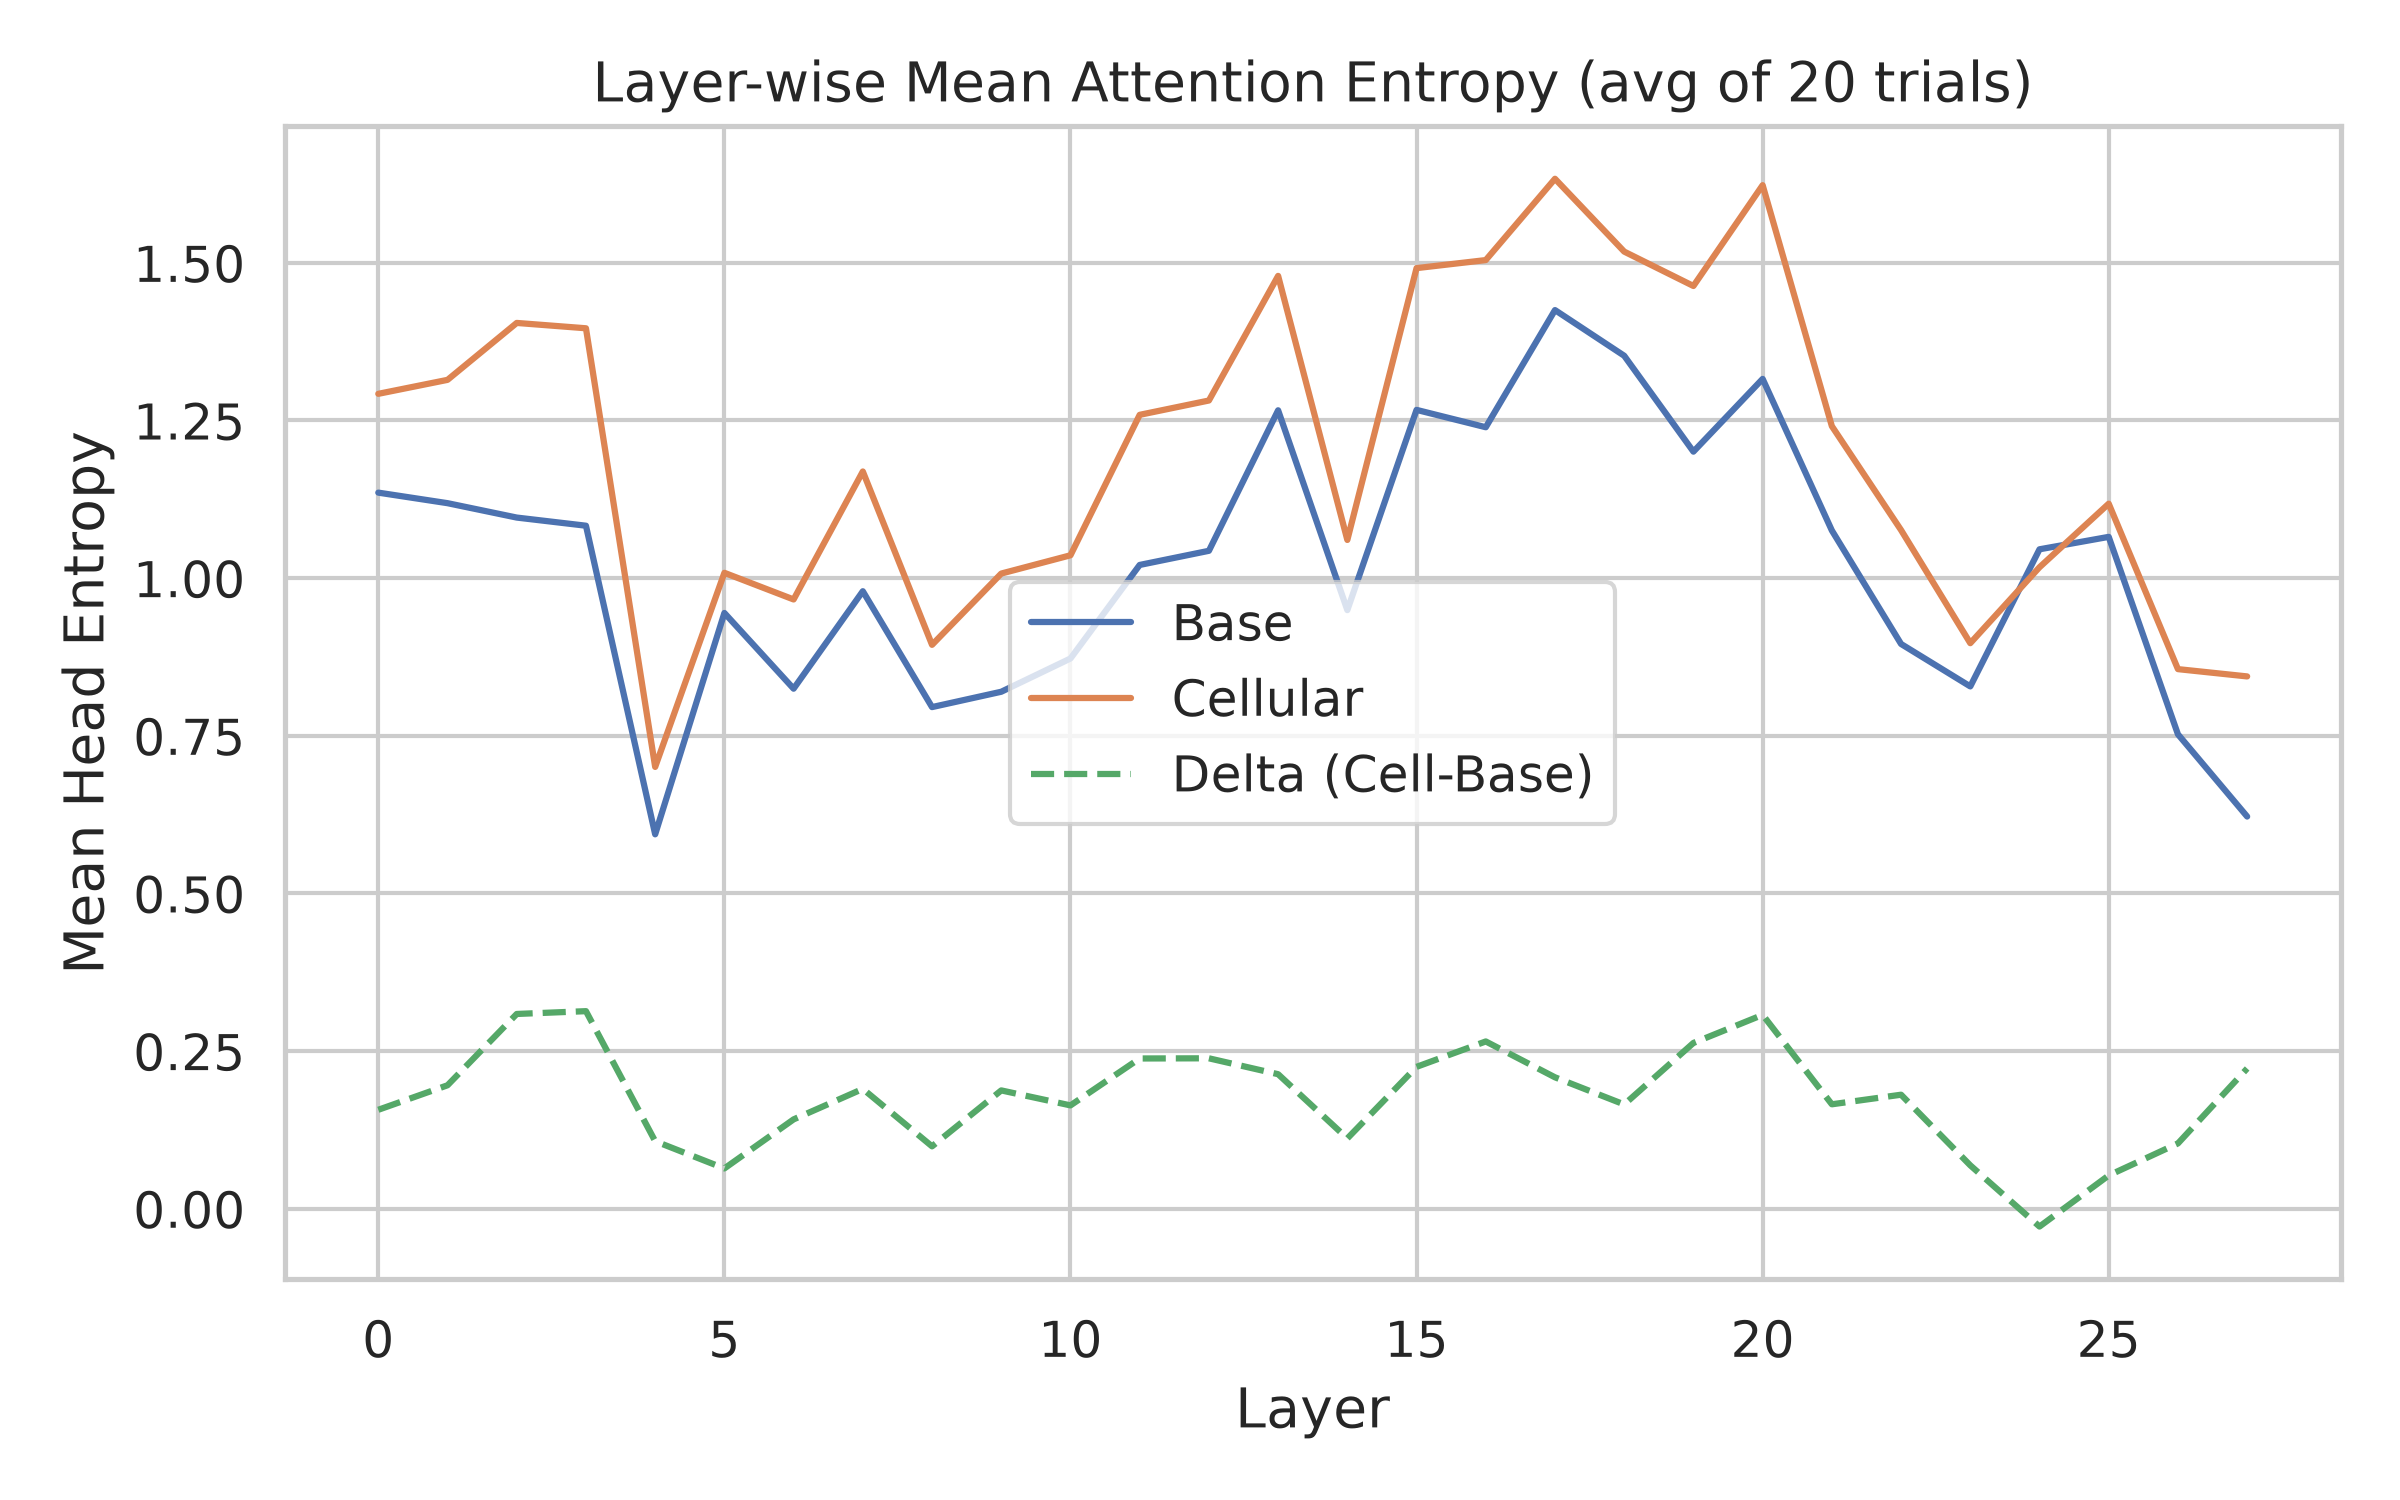
\includegraphics[width=\textwidth]{figures/fig13.png}
  \caption{Mean attention entropy by layer, Base vs.\ Cellular, 20-trial average.}
  \label{fig:fig13}
\end{figure}

\begin{figure}[htbp]
  \centering
  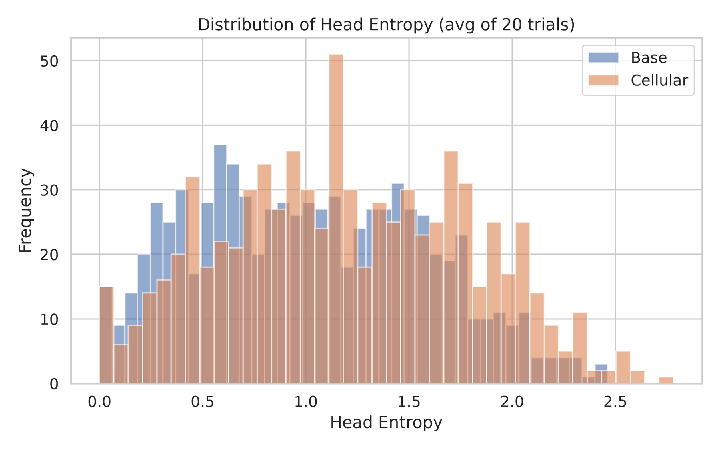
\includegraphics[width=0.7\textwidth]{figures/fig14.png}
  \caption{The same entropy values as Figure~\ref{fig:fig13}, pooled across every layer and head.}
  \label{fig:fig14}
\end{figure}

An earlier version of this analysis used one illustrative example rather than an average, and that specific draw happened to show entropy going in the \emph{opposite} direction from what the mechanism would predict (Cellular \emph{lower} than Base). Rebuilding it as a genuine 20-trial average at the identical configuration resolved this cleanly: mean entropy is Base $= 1.022$ vs.\ Cellular $= 1.198$, with Cellular higher in 27 of 28 layers --- closely matching this project's own 360-trial statistical sweep at the identical configuration (Base $= 1.020$, Cellular $= 1.197$, Cellular higher in 20 of 20 trials), and the broader sweep across every tested sequence length is unambiguous: \textbf{Cellular has higher entropy than Base in 360 of 360 trials} (mean Base $= 1.511$, Cellular $= 1.630$). We report the single-example failure explicitly here as a demonstration of why every mechanistic claim in this study was ultimately checked against a multi-trial statistic rather than left as a single anecdote.

\subsection{Off-diagonal attention and distance decay}
\label{sec:distance-decay}

\begin{figure}[htbp]
  \centering
  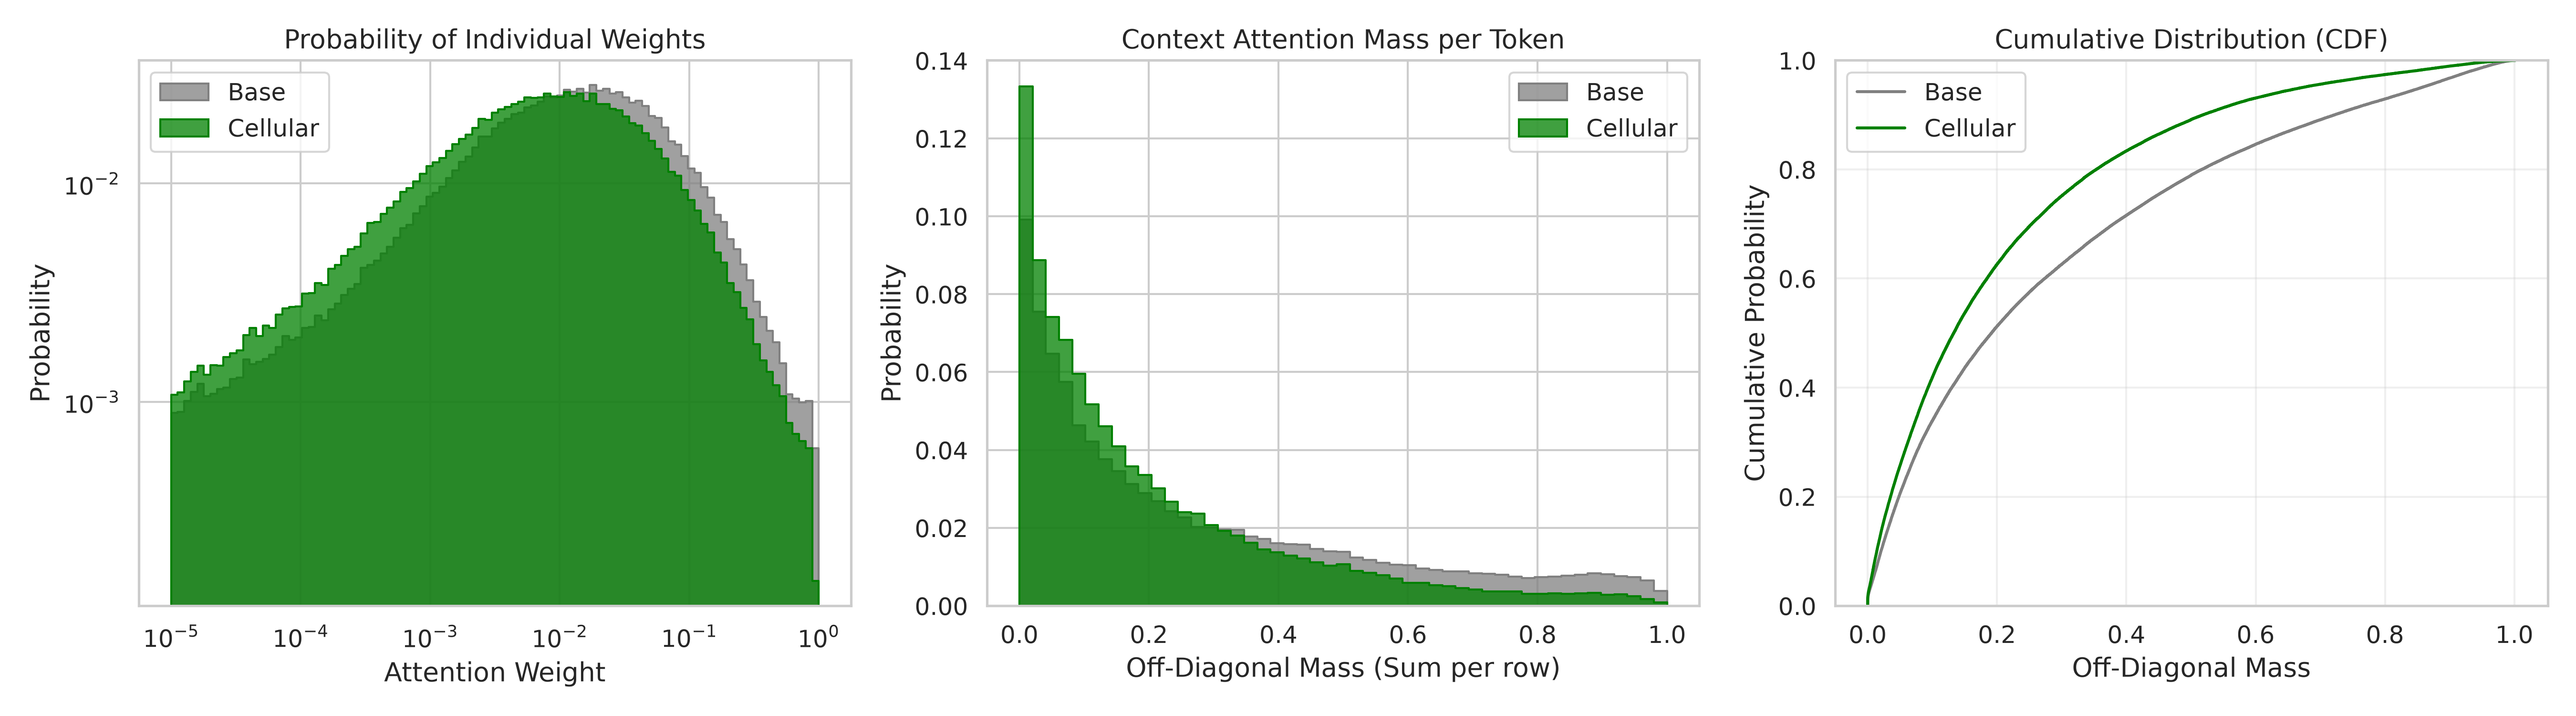
\includegraphics[width=\textwidth]{figures/fig15.png}
  \caption{Off-diagonal attention weight distributions (individual weights, per-token mass, CDF), pooled across 20 trials.}
  \label{fig:fig15}
\end{figure}

Cellular's mean off-diagonal attention mass is lower than Base's (0.207 vs.\ 0.284) --- attention under boundaries is, on net, more concentrated near the diagonal, consistent with the original proposal's description of a ``leftward shift'' toward lower-magnitude weights. A genuine wrinkle appears in a related but distinct metric: attention-\emph{weighted average distance} actually goes the other way, with Cellular reaching slightly \emph{further} on average (0.068 vs.\ 0.065, in 330 of 360 sweep trials). These are not in conflict: Cellular spends less total attention off the diagonal, but some of what it does spend is reaching specifically for boundary tokens sitting a moderate distance back, which pulls the average distance up even as overall spread shrinks.

\begin{figure}[htbp]
  \centering
  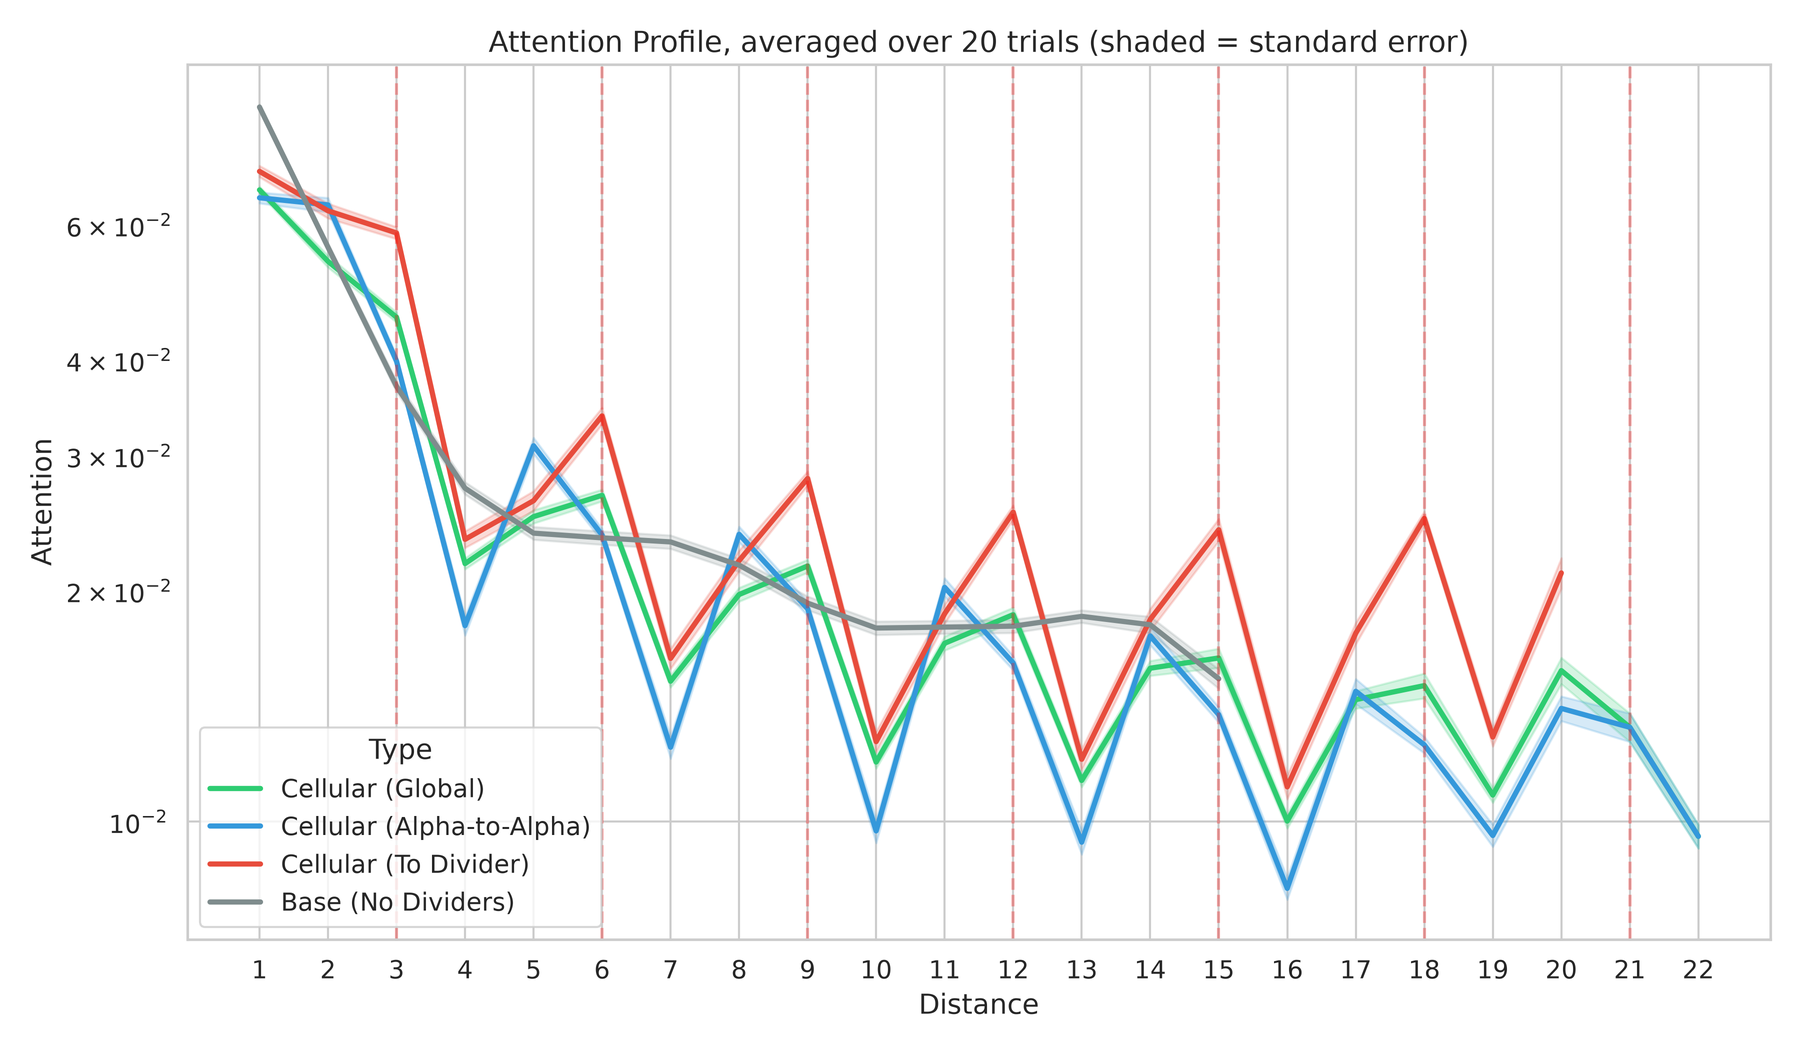
\includegraphics[width=\textwidth]{figures/fig16.png}
  \caption{Mean attention weight vs.\ token distance, split into global / to-boundary / letter-to-letter attention, 20-trial average with SEM bands.}
  \label{fig:fig16}
\end{figure}

Letter-to-letter attention dips visibly at every distance that is an exact multiple of the raw token periodicity boundaries introduce (every third position at $k=2$, since two letters plus one boundary token repeats with period 3), while Base's attention (no boundaries at all) declines smoothly with no such structure. This is the clearest position-level confirmation that boundaries interrupt letter-to-letter attention specifically at the positions where they sit, now backed by 20 trials with visible standard-error bands rather than one noisy example.

\subsection{The cost of the cheap approximation: boundaries vs.\ true divide-and-conquer}
\label{sec:divide-conquer}

\begin{figure}[htbp]
  \centering
  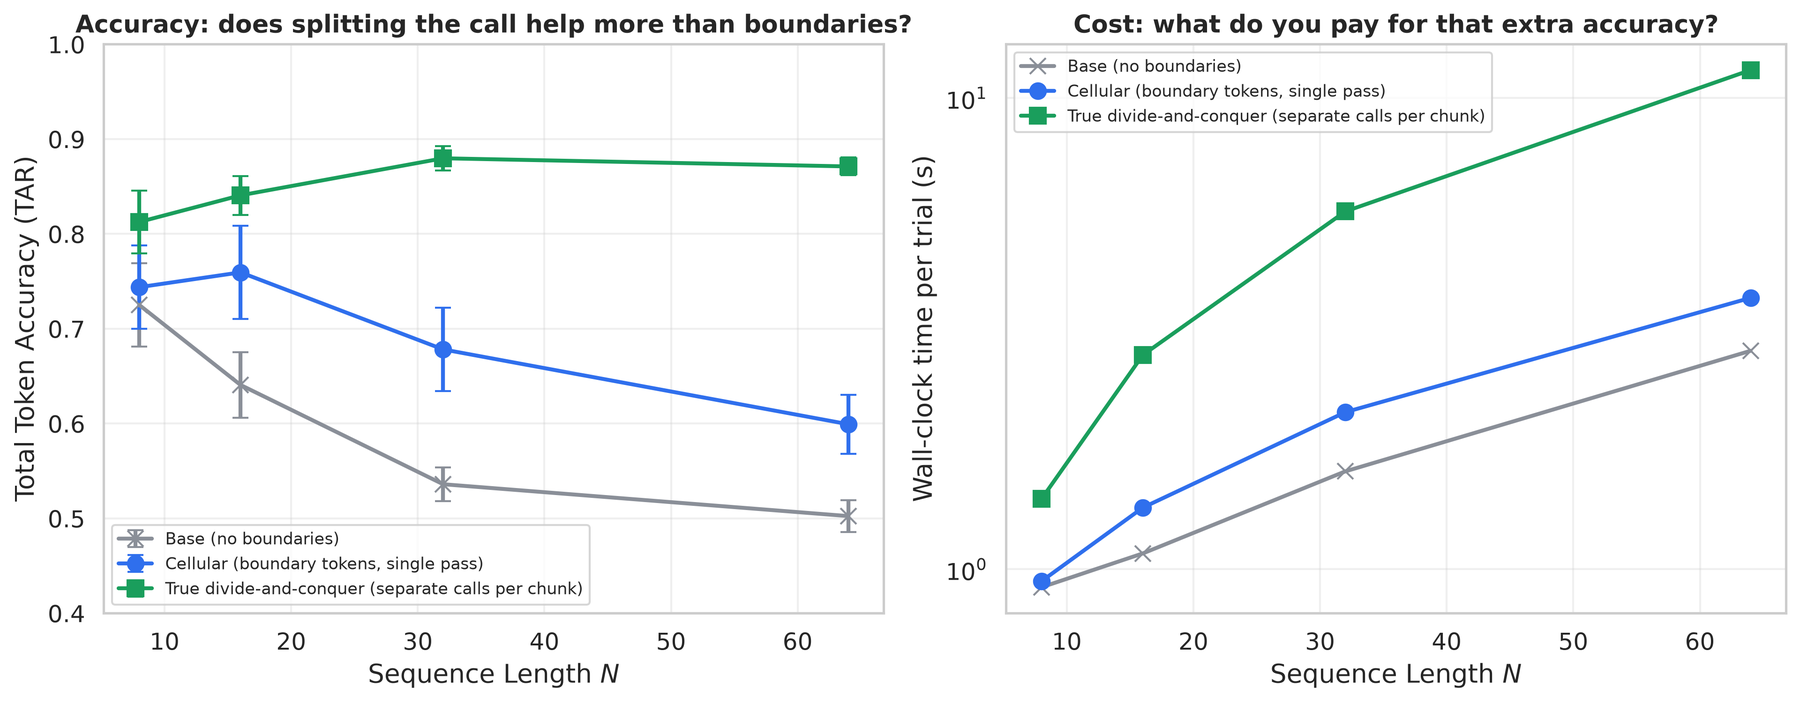
\includegraphics[width=\textwidth]{figures/fig17.png}
  \caption{Cyclic shift (alphabet=2), Qwen2.5-7B: TAR (left) and wall-clock time per trial (right, log scale) for Base, Cellular (single-pass boundary tokens), and true divide-and-conquer (the sequence actually split into separate model calls per chunk, merged after).}
  \label{fig:fig17}
\end{figure}

True divide-and-conquer wins on accuracy at every tested length, and its advantage \emph{grows} with $N$ rather than shrinking: TAR of $0.812 \rightarrow 0.841 \rightarrow 0.880 \rightarrow 0.871$ at $N = 8/16/32/64$, essentially flat-to-improving, while Cellular's TAR ($0.744 \rightarrow 0.759 \rightarrow 0.678 \rightarrow 0.599$) degrades over the same range. But this comes at a real and growing compute cost: divide-and-conquer takes $1.5\times$ as long as Base at $N=8$, climbing to $3.0\times$ the cost of Cellular ($3.9\times$ the cost of Base) by $N=64$, since it requires re-processing the prompt from scratch for every chunk rather than in one pass. Structural boundary tokens recover a substantial fraction of divide-and-conquer's accuracy benefit --- clearly beating Base through $N=32$ --- for close to Base's own compute cost. This is the direct empirical version of the efficiency argument motivating the whole approach: boundaries are a cheap, single-pass approximation to a more expensive but more effective multi-call strategy, not a replacement for it.

\textbf{Implementation details.} Chunks are fixed at 4 characters (matching the boundary-ablation grid's interval=4 condition), non-overlapping, generated independently via separate \texttt{model.generate()} calls on the same single A100 GPU used for every other local-model experiment, and concatenated directly with no re-ranking or boundary-stitching correction --- cyclic shift's per-position independence makes stitching trivial. This would not be expected to generalize as-is to tasks with cross-chunk dependency (e.g. addition), which is precisely why boundaries and true divide-and-conquer are compared on cyclic shift only here, not on the negative-result tasks. Wall-clock time is measured per-call via \texttt{time.perf\_counter()} around each \texttt{generate()} invocation and summed across a trial's chunks for divide-and-conquer; no batching is used for any of the three conditions, so all three costs are directly comparable call-for-call on identical hardware.

\subsection{Uncertainty in the $\alpha$ estimates}
\label{sec:bootstrap-ci}

Every $\alpha$ reported so far is a point estimate from a single nonlinear fit, and Fig.~\ref{fig:fig1} additionally averages across boundary densities --- both are worth stress-testing directly rather than taking on faith. We bootstrapped every (model, density) fit at alphabet=2 (resampling the 20 trials at each tested length with replacement, refitting, 500 iterations per condition; full results in \texttt{results/alpha\_bootstrap\_ci.csv}).

Two things fall out cleanly. First, \textbf{Base condition $\alpha$ is genuinely underconstrained}: 95\% CIs span $[1.02, 2.18]$ for Qwen2.5-7B, $[1.05, 2.24]$ for Qwen2.5-14B, and $[1.51, 2.12]$ for Mistral-7B --- wide intervals, consistent with SAR collapsing to floor by $N\geq 64$ and leaving few informative points to pin down the fit. Second, \textbf{the well-populated Cellular densities that carry the headline claim are considerably better constrained}: Qwen2.5-7B at $k=1$ gives $\alpha=1.037$, 95\% CI$=[1.019, 1.084]$, comfortably below Base's own lower bound; Qwen2.5-14B at $k=2$ gives $\alpha=1.153$, CI$=[1.133, 1.164]$. The reduction in $\alpha$ from Base to Cellular is not just a point-estimate artifact for these specific, well-supported conditions.

The bootstrap also validates a caution already flagged qualitatively (Section~\ref{sec:results-headline}): fits pinned against the optimizer's lower bound ($\alpha\approx 1.000$) turn out to have exactly the unstable behavior that flag was meant to signal --- Qwen2.5-7B at $k=3$ gives a 95\% CI of $[1.000, 1.679]$, and Qwen2.5-14B at $k=3$ and $k=4$ show the same pattern. These should be read as ``the cliff is very flat or absent here,'' never as a precise measurement, exactly as originally stated --- the bootstrap just confirms that caution was warranted rather than overcautious.

Table~\ref{tab:alpha-beta0} reports every fitted $(\beta_0, \alpha)$ pair underlying the discussion above alongside its bootstrap CI, rather than leaving the full set implicit in prose.

\begin{table}[htbp]
\centering
\small
\begin{tabular}{llrrrr}
\toprule
Model & Method & $k$ & $\beta_0$ & $\alpha$ & 95\% CI \\
\midrule
Qwen2.5-7B & Base & --- & 0.097 & 1.212 & [1.017, 2.181] \\
Qwen2.5-7B & Cellular\_Bounds & 1 & 0.005 & 1.037 & [1.019, 1.084] \\
Qwen2.5-7B & Cellular\_Bounds & 2 & 0.010 & 1.022 & [1.006, 1.068] \\
Qwen2.5-7B & Cellular\_Bounds & 3 & 0.663 & 1.000 & [1.000, 1.679] \\
Qwen2.5-7B & Cellular\_Bounds & 4 & 0.049 & 1.197 & [1.197, 1.347] \\
\addlinespace
Qwen2.5-14B & Base & --- & 0.075 & 1.258 & [1.045, 2.236] \\
Qwen2.5-14B & Cellular\_Bounds & 1 & 0.000 & 1.269 & [1.199, 1.317] \\
Qwen2.5-14B & Cellular\_Bounds & 2 & 0.000 & 1.153 & [1.133, 1.164] \\
Qwen2.5-14B & Cellular\_Bounds & 3 & 0.125 & 1.000 & [1.000, 1.003] \\
Qwen2.5-14B & Cellular\_Bounds & 4 & 0.149 & 1.000 & [1.000, 1.323] \\
Qwen2.5-14B & Cellular\_Bounds & 8 & 0.028 & 1.135 & [1.111, 1.135] \\
\addlinespace
Mistral-7B-v0.3 & Base & --- & 0.035 & 1.781 & [1.508, 2.121] \\
Mistral-7B-v0.3 & Cellular\_Bounds & 1 & 0.045 & 1.054 & [1.005, 1.341] \\
Mistral-7B-v0.3 & Cellular\_Bounds & 2 & 0.236 & 1.345 & [1.251, 1.552] \\
Mistral-7B-v0.3 & Cellular\_Bounds & 3 & 0.091 & 1.178 & [1.000, 2.121] \\
Mistral-7B-v0.3 & Cellular\_Bounds & 4 & 0.062 & 1.246 & [1.197, 1.274] \\
\bottomrule
\end{tabular}
\caption{Fitted SK parameters and 500-iteration bootstrap 95\% CIs for $\alpha$, alphabet=2, every (model, density) condition with a valid fit. Full data in \texttt{results/alpha\_beta0\_table.csv}.}
\label{tab:alpha-beta0}
\end{table}

\subsection{Is boundary attention necessary, not just correlated with the benefit?}
\label{sec:causal-ablation}

Every mechanistic result so far (Sections~\ref{sec:attention-sinks}--\ref{sec:distance-decay}) is correlational: boundary attention mass rises with density, and density correlates with lower $\alpha$, but nothing establishes that this attention pattern is actually \emph{load-bearing} for the accuracy benefit rather than a side effect that happens alongside it. We tested this causally (methodology in Section~\ref{sec:mechanistic-methods}): identify the 10 (of 784) attention heads in Qwen2.5-7B with the highest mean attention mass on boundary tokens via a fresh diagnostic pass, then re-run the headline condition (alphabet=2, $k=2$) with attention from exactly those heads to boundary-token positions zeroed post-softmax and renormalized, leaving every other head and every other attended position untouched. The 10 target heads are concentrated in specific layers rather than spread evenly (top mass: layer 15/head 5, layer 1/head 24, layer 3/heads 22, 24, and 25, layer 0/head 6, layer 16/head 21, layer 21/heads 6 and 9, layer 22/head 5), consistent with the scattered, non-uniform layer clustering already seen in the correlational per-head breakdown (Figure~\ref{fig:fig12}).

\begin{figure}[htbp]
  \centering
  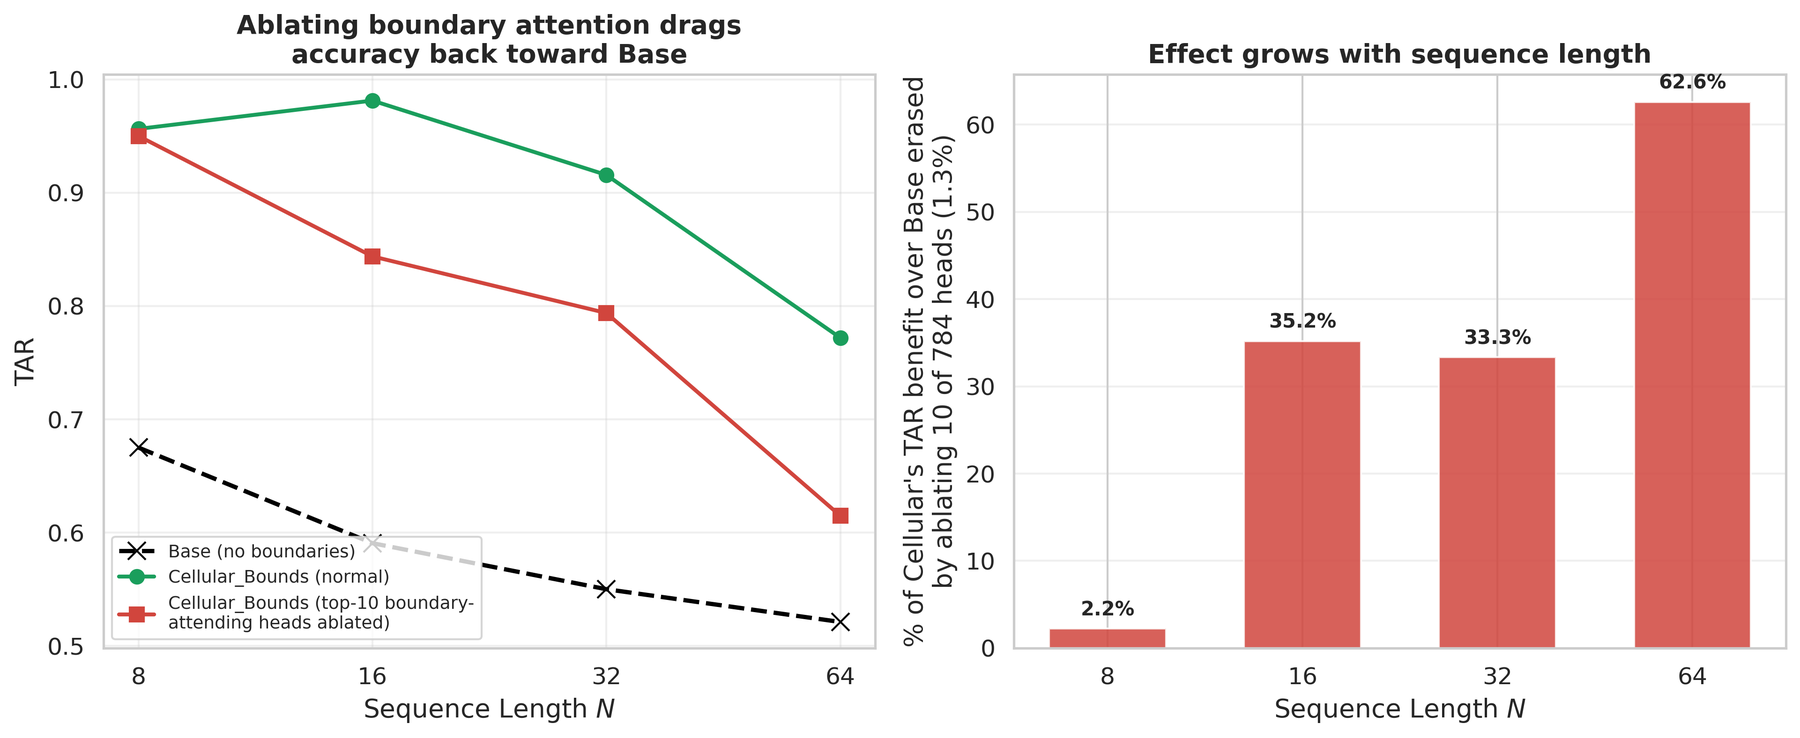
\includegraphics[width=\textwidth]{figures/fig19.png}
  \caption{Left: TAR vs.\ sequence length for Base, normal Cellular\_Bounds, and Cellular\_Bounds with the top 10 boundary-attending heads ablated. Right: the percentage of Cellular's TAR benefit over Base that ablation erases, by length.}
  \label{fig:fig19}
\end{figure}

Ablating just 1.3\% of the model's attention heads --- and only their attention to boundary-token positions specifically, nothing else --- drags accuracy substantially back toward Base, and the size of that drag grows with sequence length: 2.2\% of Cellular's TAR benefit over Base is erased at $N=8$, climbing to 35.2\% at $N=16$, 33.3\% at $N=32$, and 62.6\% at $N=64$. At the longest tested length, ablating ten heads' access to boundary tokens alone erases nearly two-thirds of the entire benefit boundary tokens provide. This is direct causal evidence, not merely correlational, that the attention-sink mechanism proposed in this line of work is functionally necessary for the accuracy gain, at least for the small subset of heads that carry most of the boundary-attention mass --- and the fact that the effect strengthens with $N$ mirrors the same length-dependence already seen in the purely correlational boundary-attention-mass result (Figure~\ref{fig:fig3}), reinforcing that this is the same mechanism being measured two different ways.

\subsection{A fourth model family: Phi-3.5-mini-instruct}
\label{sec:fourth-model}

The three models above span two architecture families (Qwen, Mistral) at two parameter scales, but all sit in a similar 7--14B range. We additionally tested \textbf{Phi-3.5-mini-instruct} (3.8B parameters, Microsoft's Phi family), a genuinely different and substantially smaller architecture, on the identical grid, seeds, and task logic as the other three models. Llama-3.1-8B-Instruct and Gemma-2-9b-it were tried first as the two most standard choices for a fourth family, but both are gated on Hugging Face with no access granted to the project's token at the time of writing; Phi-3.5-mini-instruct is openly accessible and was used to keep this check moving.

Phi-3.5-mini-instruct turns out to be a substantially weaker model on this task overall than any of the other three. Its \textbf{Base} condition's SAR (whole-sequence exact match) already collapses to 0 by $N=16$ (0.20 $\rightarrow$ 0.05 $\rightarrow$ 0.00 at $N=4/8/16$), and Cellular\_Bounds follows the same trajectory from a higher starting point. This means the SK stretched-exponential fit used throughout this paper is not meaningfully applicable here: with SAR already at floor for both conditions well before the fit has enough non-degenerate points to work with, the fitted $\alpha$ values are curve-fit artifacts pinned against the optimizer's boundary, not genuine measurements, and we do not report them for this model. We instead report the raw accuracy curves directly.

\begin{figure}[htbp]
  \centering
  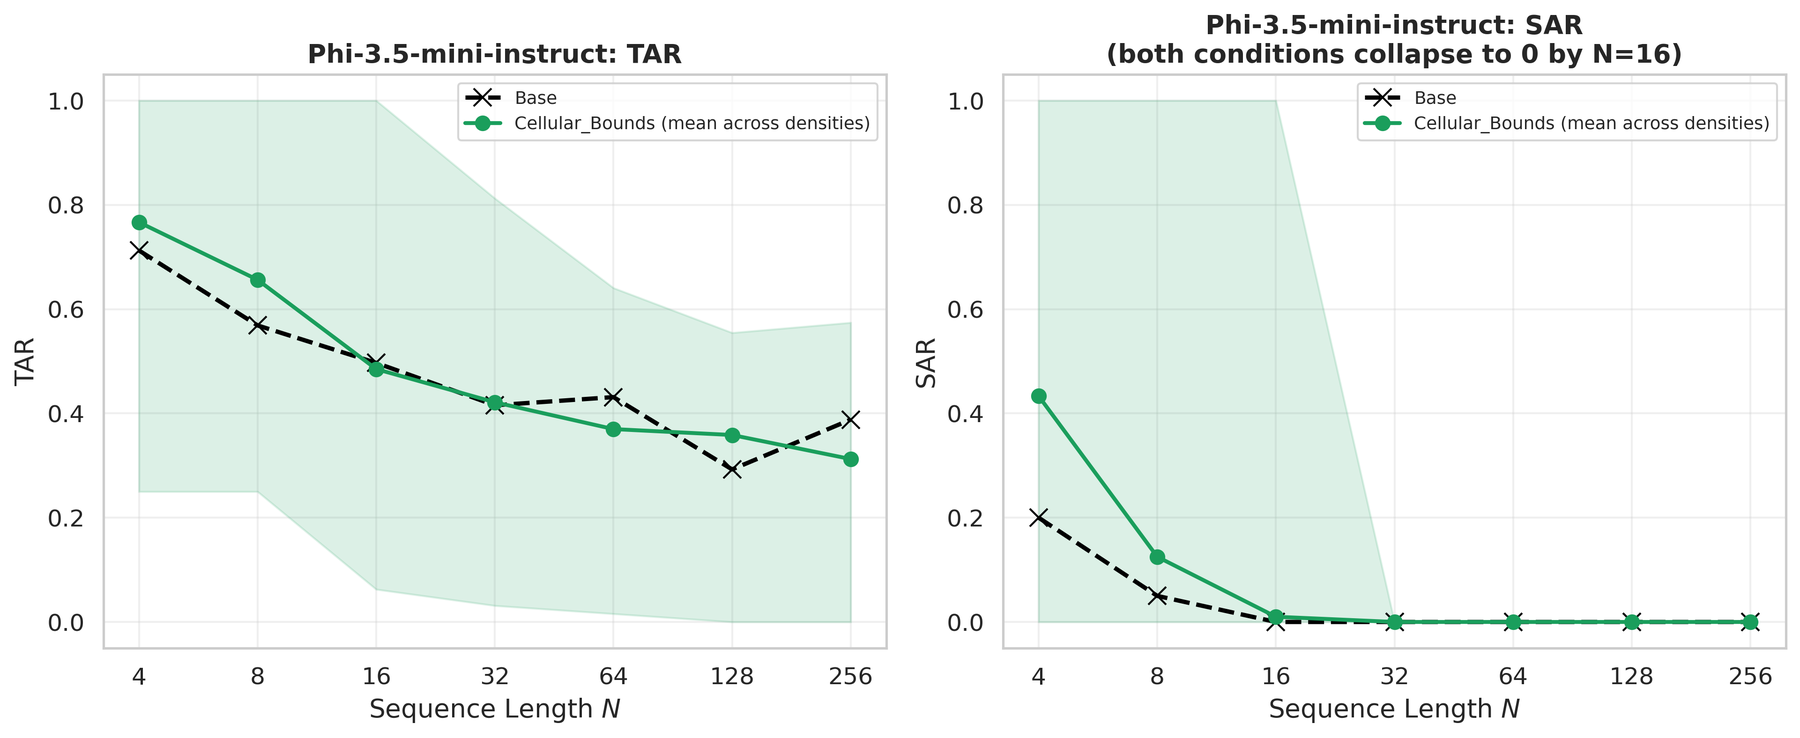
\includegraphics[width=\textwidth]{figures/fig20.png}
  \caption{Phi-3.5-mini-instruct, alphabet=2: TAR (left) and SAR (right) vs.\ sequence length, Base vs.\ Cellular\_Bounds (mean across tested densities; band = full range across densities).}
  \label{fig:fig20}
\end{figure}

Within the narrow window where the raw data is informative, the direction of the headline effect still holds: Cellular's SAR clears Base at both $N=4$ (0.433 vs.\ 0.200) and $N=8$ (0.125 vs.\ 0.050), the same direction seen in all three other models. But that separation collapses into a much narrower length window here --- both conditions are at floor by $N=16$, whereas the other three models still show a clear, measurable gap out to $N=256$ (Figure~\ref{fig:fig1B}) --- and on the coarser TAR metric, the two conditions are close to indistinguishable from $N=16$ onward and Cellular even trails Base at several longer lengths. We read this as an important boundary condition on the whole framework rather than a reversal of the core finding: the SK decay-curve comparison this paper relies on throughout requires the underlying model to have enough raw competence at the task for both conditions' decay curves to be well-resolved over a non-trivial length range. Below some minimum capability threshold, both conditions crash to floor almost immediately, and neither the accuracy comparison nor the $\alpha$-based framework has enough signal left to distinguish them cleanly.

\subsection{Does the causal-ablation mechanism matter? Pre-softmax masking vs.\ post-softmax zero-and-renormalize}

Section~\ref{sec:causal-ablation}'s causal ablation zeros attention weight to boundary positions \emph{after} softmax and renormalizes the row to still sum to 1. A cleaner-sounding alternative is to mask the raw attention score to $-\infty$ \emph{before} softmax (exactly how an ordinary causal mask works) and let softmax itself do the renormalization. These two operations are algebraically identical --- zeroing a subset of a softmax distribution's mass and renormalizing the remainder reduces to exactly the same expression as computing softmax over only the remaining positions from the start --- so this is a test of whether that equivalence actually holds in practice (bf16 rounding, implementation details) rather than an attempt to find a different result.

\begin{table}[htbp]
\centering
\small
\begin{tabular}{lrrrrr}
\toprule
$N$ & Base & Cellular (normal) & Ablated (post-softmax) & Ablated (pre-softmax) & Diff. \\
\midrule
8  & 0.675 & 0.956 & 0.950 & 0.950 & 0.000 \\
16 & 0.591 & 0.981 & 0.844 & 0.841 & $-0.003$ \\
32 & 0.550 & 0.916 & 0.794 & 0.783 & $-0.011$ \\
64 & 0.521 & 0.772 & 0.615 & 0.613 & $-0.002$ \\
\bottomrule
\end{tabular}
\caption{TAR under the two ablation mechanisms, same 10 target heads, same seeds.}
\end{table}

The two mechanisms agree to within 0.011 TAR at every length --- noise, not a systematic difference, exactly as the algebra predicts. This rules out the specific renormalization step as a confound: the causal finding in Section~\ref{sec:causal-ablation} is not an artifact of \emph{how} the ablation was implemented.

\subsection{Do the boundary-attending heads overlap with induction heads?}

Olsson et al.'s induction heads (arXiv:2209.11895) implement a ``complete the pattern'' copy operation: given a repeated sequence \texttt{... X Y ... X}, an induction head attends from the second \texttt{X} back to the position right after the \emph{first} \texttt{X} (i.e.\ copies \texttt{Y}). We tested whether the 10 heads identified as most boundary-attending (Section~\ref{sec:causal-ablation}) are also strong induction heads, using the standard operational test: 20 synthetic trials of a random 30-token chunk immediately repeated, measuring each of the model's 784 heads' attention from the second copy back to its induction target, relative to that same head's average attention to other, non-matching earlier positions (its own baseline).

\begin{table}[htbp]
\centering
\small
\begin{tabular}{rrrrr}
\toprule
Layer & Head & Boundary mass & Induction score & Induction percentile \\
\midrule
15 & 5  & 0.074 & $-0.022$ & 8.0 \\
1  & 24 & 0.072 & $-0.020$ & 17.0 \\
3  & 24 & 0.066 & $-0.018$ & 22.2 \\
3  & 22 & 0.062 & $-0.017$ & 27.6 \\
3  & 25 & 0.062 & $-0.021$ & 11.7 \\
0  & 6  & 0.061 & $-0.021$ & 13.3 \\
16 & 21 & 0.061 & $-0.016$ & 29.0 \\
21 & 9  & 0.060 & $-0.021$ & 12.3 \\
21 & 6  & 0.060 & 0.003 & 70.5 \\
22 & 5  & 0.060 & 0.295 & \textbf{97.2} \\
\bottomrule
\end{tabular}
\caption{The 10 boundary-attending target heads, ranked by induction score percentile among all 784 heads.}
\end{table}

Nine of the ten boundary-attending heads rank \emph{below} the population median induction score (mean percentile 30.9 out of 100, where 50 would mean ``indistinguishable from a random head'') --- as a population, the boundary-attending heads are not simply repurposed induction heads. But there is one clear exception: layer 22, head 5 is both a top-10 boundary-attending head \emph{and} the 3rd-strongest induction head in the entire model (97.2nd percentile). This is a genuinely mixed result: the two head populations are mostly functionally distinct, but with at least one head plausibly serving both roles, which is worth a dedicated follow-up (larger induction-test sweep, more target heads) rather than either being cleanly forced into ``yes, overlap'' or ``no, distinct.''

\subsection{Carry-aligned boundary placement for addition: a confounded negative result}

Section~\ref{sec:addition}'s addition boundaries are inserted at a fixed character interval over the flat \texttt{A\_digits + B\_digits} string, slicing through digit-column pairs arbitrarily with no relationship to where carries actually propagate. We tested a placement aligned to the task's real computational structure instead: the two operands interleaved by column, each boundary grouping exactly one addition column's two digits (\texttt{A0B0|A1B1|...|A(N-1)B(N-1)}), so a carry step's inputs are never split across a boundary.

\begin{table}[htbp]
\centering
\small
\begin{tabular}{rrrr}
\toprule
$N$ & Base & Best fixed-interval Cellular & Carry-aligned \\
\midrule
4  & 0.750 & 0.550 & 0.075 \\
8  & 0.812 & 0.256 & 0.062 \\
16 & 0.694 & 0.566 & 0.012 \\
32 & 0.631 & 0.131 & 0.014 \\
64 & 0.502 & 0.124 & 0.003 \\
\bottomrule
\end{tabular}
\end{table}

This does not rescue the effect --- it makes things dramatically worse, collapsing to near-zero TAR at every length. But inspecting the raw responses shows why this comparison is confounded rather than a clean test of carry alignment: the model's response length stays flat at roughly 4.2--4.3 characters regardless of $N$ (4, 8, 16, 32, or 64), instead of scaling with the task. The interleaved-column format is simply unfamiliar enough that the model appears unable to parse the task at all, independent of any carry-alignment benefit the placement might otherwise offer. We report this as an honest negative result with a clear caveat: this specific operationalization does not isolate carry-alignment from format-unfamiliarity, and a cleaner test would need to preserve the model's familiar \texttt{A + B} presentation while only moving boundary positions within it --- left as a concrete direction for follow-up rather than a settled answer.

\subsection{A real special token as boundary marker: a stronger negative result than any printable character}

Every marker tested so far (Section~\ref{sec:results-headline}) is a printable character. We tested \texttt{<|object\_ref\_start|>} --- a genuine special token already in Qwen2.5-7B-Instruct's vocabulary (reserved for Qwen2.5-VL's vision-grounding use case, structurally inert for this model's text-only chat template), inserted inline as the boundary marker at the same fixed interval as the existing marker-identity ablation.

\begin{table}[htbp]
\centering
\small
\begin{tabular}{rrrr}
\toprule
$N$ & Base & Mean printable-marker & Special-token \\
\midrule
8  & 0.725 & 0.717 & 0.469 \\
16 & 0.584 & 0.729 & 0.216 \\
32 & 0.538 & 0.666 & 0.092 \\
64 & 0.522 & 0.614 & 0.049 \\
\bottomrule
\end{tabular}
\end{table}

The special token does not just underperform printable markers --- from $N=16$ on, it underperforms \emph{Base itself}, the only marker in this entire study (besides the natural-token short-length exception in Section~\ref{sec:results-headline}) to do so this severely. Inspecting raw responses reveals a distinct failure mode from every other marker tested: mean response length stays flat at roughly 4.2 characters regardless of $N$ (8, 16, 32, or 64), rather than scaling with task length --- the model's generation appears to be derailed almost immediately, not merely producing a wrong but appropriately-sized answer. This is consistent with a real out-of-band special token carrying strong enough associations from its actual training use (vision grounding) that inserting it into an unrelated text task actively disrupts normal generation, unlike the printable characters tested throughout the rest of this paper, which serve as a genuinely neutral structural signal.

\subsection{Cross-model mechanistic replication: does the mechanism hold beyond Qwen2.5-7B?}
\label{sec:cross-model-replication}

Every mechanistic result up to this point (attention-sink scaling, entropy, causal ablation) was established on a single model. We replicated the full mechanistic battery --- the 420-condition attention-sink/entropy sweep and the causal ablation --- on Qwen2.5-14B and Mistral-7B-v0.3, at the identical configurations (alphabet=2, matched seeds).

\textbf{The correlational findings replicate cleanly on both models.} Boundary-attention mass scales with density ($1/k$) with $R^2 \geq 0.97$ at every one of the 6 tested lengths for both Qwen2.5-14B and Mistral-7B (matching Qwen2.5-7B's $R^2 \geq 0.98$), and attention entropy is higher under Cellular\_Bounds than Base in 360 of 360 sampled trials for \emph{both} models --- exactly the same unanimous result already reported for Qwen2.5-7B in Section~\ref{sec:entropy-catch}.

\textbf{The causal finding replicates in direction but not in magnitude, and the picture is genuinely mixed.} On Qwen2.5-14B, ablating the top 10 boundary-attending heads drags TAR toward Base with the same growing-with-length pattern seen on 7B, but far more weakly: 0\%, 0\%, 3.8\%, and 15.8\% of Cellular's benefit erased at $N=8/16/32/64$, versus 7B's 2.2\%/35.2\%/33.3\%/62.6\%. This is not necessarily a weaker mechanism --- 14B's Cellular\_Bounds condition is already at or near ceiling (99.4--100\% TAR) at this density for most lengths, leaving little headroom for any intervention to move it, causal or otherwise. On Mistral-7B, the ablation effect is noisy and inconsistent (a small negative effect at $N=8$, a small \emph{positive} effect at $N=16$, none at $N=32$, and a large apparent positive effect at $N=64$) --- but this reflects a different confound: Mistral's own Cellular\_Bounds benefit at this specific density ($k=2$) is already tiny to begin with (Section~\ref{sec:bootstrap-ci}'s own bootstrap results show Mistral's $k=2$ condition is one of its weaker densities, $\alpha=1.345$ vs.\ Base's $1.781$), so the ``percentage of benefit erased'' metric divides by a small, noisy denominator and becomes unstable. A fairer causal test on Mistral would repeat this at a density where Mistral's own correlational benefit is actually strong (e.g.\ $k=1$, $\alpha=1.054$) --- left as a direction for follow-up rather than run here.

The honest summary: the \emph{correlational} mechanism (attention sinks, rising entropy) is now confirmed as a general property across all three models in this study, not an artifact of one. The \emph{causal} confirmation (Section~\ref{sec:causal-ablation}) is real and directionally consistent on the one other model where it's cleanly measurable (14B), but its magnitude depends heavily on how much headroom is left in that model's own accuracy at the tested density --- a caution about generalizing a specific causal-effect-size number, not about the mechanism's existence.

\section{Discussion}
\label{sec:discussion}

\textbf{What is robust.} Boundaries substantially and consistently reduce error-accumulation for the simplest task variant (2-symbol alphabet), across three models spanning two architectures and two parameter scales. This is backed by a real, checkable mechanism: boundary tokens measurably absorb attention ($R^2 \geq 0.97$--$0.98$), that absorption grows with density and --- more slowly --- with sequence length, attention entropy rises under boundaries with no exceptions across 360 sampled trials, and letter-to-letter attention measurably dips at exactly the positions boundaries occupy. Both of these correlational findings now replicate cleanly on all three models in this study, not just one (Section~\ref{sec:cross-model-replication}). Critically, the mechanism is also confirmed causally rather than only correlationally (Section~\ref{sec:causal-ablation}): ablating attention to boundary tokens for just the 10 heads (of 784) that attend to them most erases up to 62.6\% of Cellular's accuracy benefit at the longest tested length on Qwen2.5-7B, with the effect strengthening as sequences get longer; the same direction replicates on Qwen2.5-14B, though far more weakly, since 14B's Cellular condition is already near ceiling at this density and has little headroom left to move (Section~\ref{sec:cross-model-replication}). The effect does not depend on the specific marker character used, extending naturally to multi-character markers as well (Section~\ref{sec:results-headline}), is not an artifact of one instruction phrasing, and the intervention is measurably cheaper than the true divide-and-conquer alternative it approximates (Section~\ref{sec:divide-conquer}): true divide-and-conquer wins on accuracy at every tested length, but at 3--4$\times$ the compute cost by $N=64$, while boundaries recover much of that accuracy benefit for close to Base's own cost.

\textbf{What is not robust.} The effect does not generalize cleanly to harder task variants. Across two harder alphabets in three models, it holds in three of six cases and reverses in the other three, with no principled account yet for which cases reverse. It also does not transfer to tasks with genuine long-range state --- running-sum-mod-$M$ shows no boundary-adjacent recovery advantage at all, and integer addition shows boundaries actively hurting at every tested length, plausibly because carries propagate in the opposite direction from generation. Reversing digit order to align carry direction with generation order did not fully rescue the effect, and allowing the model an explicit reasoning scratchpad before committing to an answer produced an inconclusive result (more than half of trials did not even yield a scoreable output in the expected format). A third, structurally different benchmark task (Pauli string multiplication, chosen to combine a position-local component with a genuinely global one within a single task) was also inconclusive: the model did not once get the position-local component fully correct across the entire sweep, and overall accuracy under boundaries was worse than Base at three of four tested lengths in the most-corrected version of the data. A fourth model family, Phi-3.5-mini-instruct, adds a further boundary condition rather than a counter-example: this smaller, weaker model's accuracy collapses to floor so quickly in \emph{both} conditions that neither the raw-accuracy comparison nor the SK fit has enough length range left to cleanly resolve the effect one way or the other (Section~\ref{sec:fourth-model}) --- a caution that the framework requires a baseline level of model competence at the task before it can be evaluated at all, distinct from the effect itself failing to hold.

We also directly tested the specific mechanistic hypothesis that boundaries should increase attention \emph{clustering} (the intuitive idea that periodicizing context into semi-independent cells should raise graph-theoretic modularity of the attention pattern). The data show the opposite, with strong statistical support ($R^2 = 0.66$--$0.76$, $p < 10^{-14}$ at every sequence length from $N=16$ to $N=256$): clustering coefficient \emph{decreases} under boundaries as density increases. We report this plainly as a case where a plausible-sounding mechanistic hypothesis, derived from the same intuition that motivates the whole intervention, did not survive contact with the data --- attention sinks and rising entropy are real and well-supported; the clustering account of \emph{why} is not, at least not in the form we tested it.

\textbf{Methodological caution.} The chat-template correction is, in our view, as important a finding as any accuracy result in this paper. It changed at least one condition (8-symbol alphabet) from noisy and inconsistent to smooth and interpretable, and it is the kind of error that would not announce itself --- the model still produces plausible-looking text either way. Any future work evaluating instruction-tuned models on structured, deterministic tasks should verify the prompting format matches what the model was actually trained on before drawing conclusions from accuracy differences between conditions.

\section{Conclusion}

Periodic structural boundary tokens measurably reduce error-accumulation and delay the accuracy cliff --- but as a real, mechanistically-grounded, and \emph{scoped} finding, not a universal one. The effect is strong and highly reproducible on the simplest task variant, across model scale and architecture family, and is backed by convergent mechanistic evidence at the attention level: boundary tokens act as attention sinks, entropy rises under boundaries with no exceptions in 360 sampled trials, and letter-to-letter attention measurably interrupts at exactly the positions boundaries occupy. The same intervention does not reliably help --- and can actively hurt --- on harder task variants and on tasks with genuine long-range state, most clearly on integer addition, where it hurts at every tested length. The honest, publishable claim is the narrower one: this is a real, cheap, mechanistically-understood intervention for the class of tasks where each output position is otherwise independent of the others, not a general-purpose fix for the accuracy cliff.

\appendix

\section{Prompt templates used in the robustness check (Section~\ref{sec:prompt-robustness})}
\label{app:prompts}

\subsection*{original}
\begin{verbatim}
You are a deterministic sequence transformer.
Task: Cyclic character shift.
Alphabet: A, B
Rule: Replace every character with the next one in the alphabet.
Mapping: B -> A, and A -> B.
Constraint: The input contains vertical bars (|). These are structural
boundaries. DO NOT shift them. Copy them exactly to the output.
No spaces, no explanations.

Input: {input}
Output:
\end{verbatim}

\subsection*{paraphrase\_1}
\begin{verbatim}
You perform one job only: shifting letters forward in a fixed alphabet.
Letters in use: A, B
For every letter you see, write the next letter in this list instead
(wrapping from B back to A).
Some characters in the input are pipes (|); these are dividers, not
letters -- reproduce them unchanged in your answer.
Respond with the transformed string only. Do not add spaces or commentary.

Sequence: {input}
Result:
\end{verbatim}

\subsection*{paraphrase\_2}
\begin{verbatim}
Apply a fixed substitution cipher: B -> A -> A.
In plain terms, replace each symbol with the one that follows it in A, B,
cycling back to the start after the last symbol.
Any "|" characters present must be left exactly where they are -- they
are not part of the alphabet.
Give only the resulting string, with no spaces and no explanation of
your reasoning.

>>> {input}
<<<
\end{verbatim}

\section{Follow-up prompts and results for integer addition (carry-direction and scratchpad)}
\label{app:addition-followups}

Two follow-up checks on the addition negative result (Section~\ref{sec:addition}): does reversing digit order to match carry direction to generation direction help, and does letting the model reason step-by-step before committing to an answer help. Neither fully rescued the effect; both are reported here in full rather than just summarized, per reviewer request.

\subsection*{Carry-direction (least-significant-digit-first) prompt}
\begin{verbatim}
You are a deterministic arithmetic calculator.
Task: Add two {length}-digit numbers. Both input numbers and the expected
output are written LEAST-SIGNIFICANT-DIGIT FIRST (reversed order, i.e.
the ones digit comes first).
Constraint: The input may contain vertical bars (|) as structural
boundaries -- they carry no numeric meaning, ignore them when computing.
Output ONLY the {length}-digit sum, also least-significant-digit-first.
No spaces, no explanations.

Input: {input}
Output:
\end{verbatim}

\begin{center}
\begin{tabular}{@{}lccc@{}}
\toprule
$N$ & Base TAR & Cellular TAR & Gap \\
\midrule
4  & 0.325 & 0.219 & $-0.106$ \\
8  & 0.306 & 0.231 & $-0.075$ \\
16 & 0.275 & 0.149 & $-0.126$ \\
32 & 0.216 & 0.074 & $-0.142$ \\
64 & 0.198 & 0.054 & $-0.144$ \\
\bottomrule
\end{tabular}
\end{center}

Reversing digit order did not rescue the effect --- Cellular remains worse than Base at every tested length, by a similar or larger margin than the original digit order.

\subsection*{Scratchpad (explicit step-by-step reasoning) prompt}
\begin{verbatim}
You are a careful arithmetic assistant.
Task: Add two {length}-digit numbers.
Constraint: The input may contain vertical bars (|) as structural
boundaries -- they carry no numeric meaning, ignore them when computing.
First, work through the addition step by step from the rightmost
(least-significant) digit to the left, tracking the carry at each step.
Then, on its own line, write exactly:
Final Answer: <the {length}-digit sum, zero-padded if needed>

Input: {input}
\end{verbatim}

\begin{center}
\begin{tabular}{@{}lccccc@{}}
\toprule
$N$ & Base TAR & Cellular TAR & Gap & Base SAR & Cellular SAR \\
\midrule
4  & 0.317 & 0.117 & $-0.200$ & 0.133 & 0.033 \\
8  & 0.025 & 0.050 & $+0.025$ & 0.000 & 0.000 \\
16 & 0.029 & 0.072 & $+0.043$ & 0.000 & 0.000 \\
\bottomrule
\end{tabular}
\end{center}

Only 52.7\% of responses across this entire sweep contained a cleanly parseable \texttt{Final Answer:} line (scored 0 when absent, matching how a real deployment would treat a malformed response). Combined with both TAR columns already sitting near floor at $N\geq 8$ regardless of condition, this result is inconclusive rather than a clean positive or negative --- reported here in full so readers can judge the data quality themselves rather than take our summary characterization on faith.

\vfill
\noindent\rule{\textwidth}{0.4pt}

\noindent\small All figures in this document are generated directly from the project's saved results (\texttt{results/}) and share methodology with the interactive project writeup. Error bars throughout are standard error of the mean unless stated otherwise. Code and raw data available in the project repository.

\end{document}
